\documentclass[main.tex]{subfiles}

\begin{document}

% -------------------------------------------------------------------------------
\section{Logo}

\begin{figure}[h!]
    \centering
    
\includegraphics[scale=0.4]{logo_completa}
    \caption{Logo EduSyst}
\end{figure}

\begin{figure}[h!]
    \centering
    
\includegraphics[scale=0.4]{logo_icone}
    \caption{Ícone EduSyst}
\end{figure}
% -------------------------------------------------------------------------------

% -------------------------------------------------------------------------------
\section{Introdução}
A complexidade na organização de dados, a comunicação deficiente entre alunos, professores e pais, juntamente com as dificuldades na gestão acadêmica e de recursos, além dos desafios de transparência e segurança de dados, são problemas enfrentados pelas escolas no dia a dia. Para enfrentar esses desafios e otimizar a administração escolar, o EduSyst foi desenvolvido como uma solução abrangente, eficiente e segura, que integra todas as funções necessárias para melhorar o gerenciamento acadêmico e a comunicação no ambiente escolar.
% -------------------------------------------------------------------------------

% -------------------------------------------------------------------------------
\section{Descrição}

\subsection{Objetivo Geral}
O objetivo do EduSyst é oferecer um sistema integrado que permita aos alunos acessar suas notas, matérias, horários e atividades virtuais; aos professores, atribuir notas, publicar atividades e acompanhar o desempenho de suas turmas; aos responsáveis, monitorar o progresso dos alunos; e aos administradores, gerenciar de forma eficiente professores, alunos, responsáveis e turmas. O sistema busca simplificar a administração escolar, melhorar a comunicação entre todos os envolvidos e promover um gerenciamento mais eficiente e transparente.

\subsection{Abrangência do Sistema}
O EduSyst abrange a gestão de dados acadêmicos, permitindo a administração de informações dos alunos, como notas, turmas, matérias, e horários.
A plataforma inclui ferramentas para o cadastro e gerenciamento de usuários (alunos, professores, responsáveis e administradores), turmas e matérias, comunicação via chat entre usuários do sistema, geração de boletins e criação de grade horária.

Os responsáveis só possuem associação com 1 (um) aluno no sistema. Por motivos de segurança, o sistema não possui recuperação de senha ao nível usuário (Responsável, Professor e Aluno). O usuário precisa solicitar ao adminstrador a mudança de sua senha. Também incorpora mecanismos para os administradores atualizarem dinamicamente as informações institucionais e gerenciarem aspectos operacionais da escola, incluindo matrículas, turmas e a atualização de conteúdo no ambiente web. O sistema não inclui criptografia de senhas por padrão, ficando sob responsabilidade do implementador assegurar a implementação de um mecanismo de criptografia adequado.


\subsection{Atores}
Os atores são os diferentes tipos de usuários que interagem com o sistema e desempenham funções específicas. Cada ator possui responsabilidades e permissões distintas para garantir o funcionamento adequado da plataforma.

\begin{itemize}
  \item Adminstradores
  \begin{itemize}
      \item Descrição: Usuários responsáveis pela gestão do sistema, incluindo a criação, atualização e exclusão de dados relacionados a usuários, turmas e disciplinas.
      \item Atributos: ID, Nome de Usuário, Senha, E-Mail.
  \end{itemize}
  
  \item Alunos
  \begin{itemize}
      \item Descrição: Alunos matriculados na escola que utilizam o sistema.
      \item Atributos: ID, CPF, E-Mail, Nome, Data de Nascimento, Gênero, Endereço, Telefone, Curso, Turmas associadas.
  \end{itemize}
  
  \item Responsáveis
  \begin{itemize}
      \item Descrição: Pais ou responsáveis pelos alunos, que acompanham o desenvolvimento acadêmico de seu aluno associado.
      \item Atributos: ID, CPF, E-Mail, Nome, Data de Nascimento, Gênero, Endereço, Telefone, Curso, Aluno associado.
  \end{itemize}
  
  \item Professores
  \begin{itemize}
      \item Descrição: Professores que utilizam o sistema para gerenciar suas turmas e atividades acadêmicas.
      \item Atributos: ID, CPF, E-Mail, Nome, Data de Nascimento, Gênero, Endereço, Telefone, Horários e Disciplinas associadas.
  \end{itemize}
\end{itemize}
% -------------------------------------------------------------------------------

% -------------------------------------------------------------------------------
% \section{Justificativa}

% \subsection{Problemas}

% \subsection{Necessidades}
% -------------------------------------------------------------------------------

% -------------------------------------------------------------------------------
% \section{Objetivo Específico}
% -------------------------------------------------------------------------------

% -------------------------------------------------------------------------------
% \section{Análise do Ambiente Organizacional}
% \subsection{Organograma} % NÃO SEI SE VAI TER!
% \subsection{Impactos na Implantação do Sistema}

\section{Impactos na Implantação do Sistema}
O EduSyst promove uma transformação social significativa ao modernizar a gestão educacional nas escolas públicas. Ao melhorar a organização e comunicação, o sistema facilita uma educação mais acessível e personalizada, reduzindo desigualdades e fortalecendo o suporte parental.
% -------------------------------------------------------------------------------

% -------------------------------------------------------------------------------
\section{Metodologia do Desenvolvimento}
Para o desenvolvimento do EduSyst, adotamos uma abordagem colaborativa e eficiente utilizando ferramentas de gestão e controle de versão. O Google Drive foi empregado para o compartilhamento e organização de documentos, facilitando o armazenamento e o acesso aos materiais do projeto, como especificações, relatórios e documentos de design. 
O GitHub foi utilizado para o controle de versão e a colaboração no código-fonte, permitindo a integração contínua das alterações e a gestão de diferentes versões do projeto. Essa combinação de ferramentas garantiu uma coordenação eficaz entre os membros da equipe, possibilitando um desenvolvimento ágil e bem documentado do sistema. O desenvolvimento do EduSyst foi realizado em três etapas distintas, cada uma com avanços significativos:
\begin{itemize}
    \item Na primeira etapa, criamos um site estático com tela de login, utilizando Bootstrap para a construção de uma interface básica, e desenvolvemos um aplicativo desktop com funcionalidades iniciais de login para administradores e uma interface básica para operações CRUD.
    \item Na segunda etapa, implementamos a conexão com um banco de dados MySQL e transformamos o site em uma aplicação dinâmica utilizando JSP. Introduzimos o login para alunos e a capacidade de listar matérias. O aplicativo desktop foi aprimorado para incluir login de administradores, recuperação de senhas, listagem de alunos, além de permitir o cadastro, alteração e exclusão de alunos.
    \item Na terceira e última etapa, concluímos o projeto com a integração de todos os requisitos funcionais previstos. O sistema agora inclui um site público com login para professores, alunos e responsáveis, um aplicativo desktop completo para a administração do sistema escolar, e um aplicativo móvel para o acesso exclusivo de alunos e responsáveis.
\end{itemize}
% -------------------------------------------------------------------------------

% -------------------------------------------------------------------------------
\section{Minimundo}
O EduSyst enfrenta o desafio de simplificar a complexidade na organização de dados e melhorar a comunicação entre alunos, professores e pais, buscando solucionar as dificuldades na gestão acadêmica das escolas públicas de ensino médio no estado do Rio de Janeiro. Seu propósito primordial é desenvolver e implementar sistemas escolares que ofereçam uma plataforma abrangente e intuitiva para atender às variadas demandas do ambiente escolar.

No sistema escolar, anualmente dividido em quatro bimestres, os alunos podem participar de múltiplas turmas. Eles têm acesso à lista de professores e matérias atribuídas, além de gerar boletins bimestrais baseados nas notas definidas pelos professores, e acessar materiais de estudo disponibilizados pelo sistema. Os alunos possuem os atributos ID, CPF, E-Mail, Nome, Data de Nascimento, Gênero, Endereço, Telefone, Curso, além das turmas na qual ele está associado.

Os professores têm a possibilidade de listar todas as turmas que lecionam, juntamente com seus respectivos alunos e matérias atribuídas. Eles também necessitam da capacidade de atribuir notas individualmente a cada aluno em suas respectivas matérias. Eles também podem aplicar atividades para suas turmas, avaliando o desempenho de cada aluno de forma personalizada. Os professores possuem os atributos ID, CPF, E-Mail, Nome, Data de Nascimento, Gênero, Endereço, Telefone, além das turmas e disciplinas na qual ele está associado.

O EduSyst facilita a comunicação entre usuários por meio de chats de turmas. Essa funcionalidade permite que professores compartilhem informações importantes e respondam a dúvidas dos alunos de forma rápida e direta.

Os Responsáveis dos alunos têm a possibilidade de acompanhar o seu desenvolvimento, através do registro dos resultados e notas de avaliações e atividades, além da possibilidade de contactar os administradores do ambiente escolar. Os Responsáveis possuem os atributos ID, CPF, E-Mail, Nome, Data de Nascimento, Gênero, Endereço, Telefone e o aluno na qual está associado.

Por fim, os administradores do sistema desempenham um papel crucial ao gerenciar matrículas, professores, alunos, turmas, matérias, horários e notas. Além disso, têm a responsabilidade de atualizar dinamicamente as informações do site do sistema escolar. Ao cadastrar usuários (alunos e professores), os administradores definem um login de identificação para acesso à seção institucional do site.

Com funcionalidades adaptadas às necessidades de cada usuário e uma interface intuitiva, o sistema contribui para a transparência, o acompanhamento acadêmico e a otimização da administração escolar, alinhando-se aos objetivos de modernização e eficiência das escolas públicas de ensino médio no Rio de Janeiro. O EduSyst apresenta uma solução abrangente e eficiente para os desafios da gestão escolar, promovendo a organização de dados e a comunicação entre alunos, professores, responsáveis e administradores.
% -------------------------------------------------------------------------------

% -------------------------------------------------------------------------------
\section{Regras do Negócio}

\subsection{Requisitos Funcionais}
\begin{itemize}
    \item Aplicativo desktop para acesso de Administradores.
    \item Ambiente web para acesso de Professores, Alunos e Responsáveis.
    \item Aplicativo móvel para acesso exclusivo de Professores, Alunos e Responsáveis, com funcionalidades limitadas.

    \item Professores:
    \begin{itemize}
        \item Consultar matérias, alunos e turmas atribuídas.
        \item Atribuir atividades on-line.
        \item Atribuir notas aos alunos.
    \end{itemize}

    \item Alunos:
    \begin{itemize}
        \item Consultar matérias, notas, grade de horários, atividades, turmas e professores.
        \item Realizar atividades.
    \end{itemize}

    \item Administradores:
    \begin{itemize}
        \item Gerenciar matrículas, professores, alunos, turmas, matérias, responsáveis, notas e horários.
        % \item Alterar informações do site de forma dinâmica via interface gráfica (nome da escola, imagens e descrição).
        \item Imprimir informações como listagem de alunos e matérias.
    \end{itemize}

    Responsáveis:
    \begin{itemize}
        \item Acompanhar o desenvolvimento dos alunos
        \item Observar matérias, notas, grade de horários, turmas atividades e professores do aluno.
    \end{itemize}
\end{itemize}

\subsection{Requisitos Não Funcionais}
\begin{itemize}
    \item API Externa para sistema de chat.

    \item Software:
    \begin{itemize}
        \item Utilizamos os sistemas operacionais Windows 10 e Windows 11 para o desevolvimento do EduSyst e o projeto foi feito com eles em mente. 
    
        \item Execução do sistema:
        \begin{itemize}
            \item Java Development Kit (JDK) 22 para execução do sistema desktop.
            \item XAMMP 8.2.12 com Tomcat 8.5.96 e PHP 8.2.12 para criação do servidor web local do website.
            \item Java Runtime Environiment (JRE) 22 para execução do website no servidor web.
            \item MariaDB 10.4.32 e PhpMyAdmin 5.2.1 para execução e manutenção do banco de dados MySQL no servidor web.
            \item Google Chrome 128 ou similar para exibição ideal do website. 
        \end{itemize}

        \item Ambiente de Desenvolvimento:
        \begin{itemize}
            \item Apache NetBeans 22 para desenvolvimento Java Desktop, Java Web, PHP, HTML5 e CSS.
            \item Android Studio 2023.3.1 Patch 2 para desenvolvimento Android.
            \item Bibliotecas:
            \begin{itemize}
                \item MySQL Connector (JDBC) 9 para conexão do site e do sistema desktop Java com o banco de dados MySQL.
                \item O'Reilly Servlet Package (cos.jar) para envio de arquivos
                pro servidor
                \item Bootstrap para design HTML.
                \item API do MeuMural para sistema de chat.
            \end{itemize}
            \item Visual Paradigm 17 Community Edition para design de diagramas de classe.
            \item Astah UML 9.2 para design de diagramas de caso de uso (DCUs).
            \item Draw.io para design do diagrama de entidade relacionamento (DER).
            \item Overleaf (LaTeX) para preparação, edição e formatação do texto do TCC.
            \item GitHub e Google Drive Desktop para desenvolvimento em equipe, backup e versionamento.
        \end{itemize}
    \end{itemize}

    \item Hardware:
    \begin{itemize}
        \item Processador Intel® Core™ i5-5200U.
        \item 8GB Memória Ram.
        \item Monitor com resolução mínima de 1366 x 768 (desktop).
        \item Tela com resolução mínima de 720 x 1280 (mobile).
    \end{itemize}
    
\end{itemize}
% -------------------------------------------------------------------------------

% -------------------------------------------------------------------------------
\section{Diagrama de Caso de Uso Geral}
\begin{figure}[H]
    \centering
    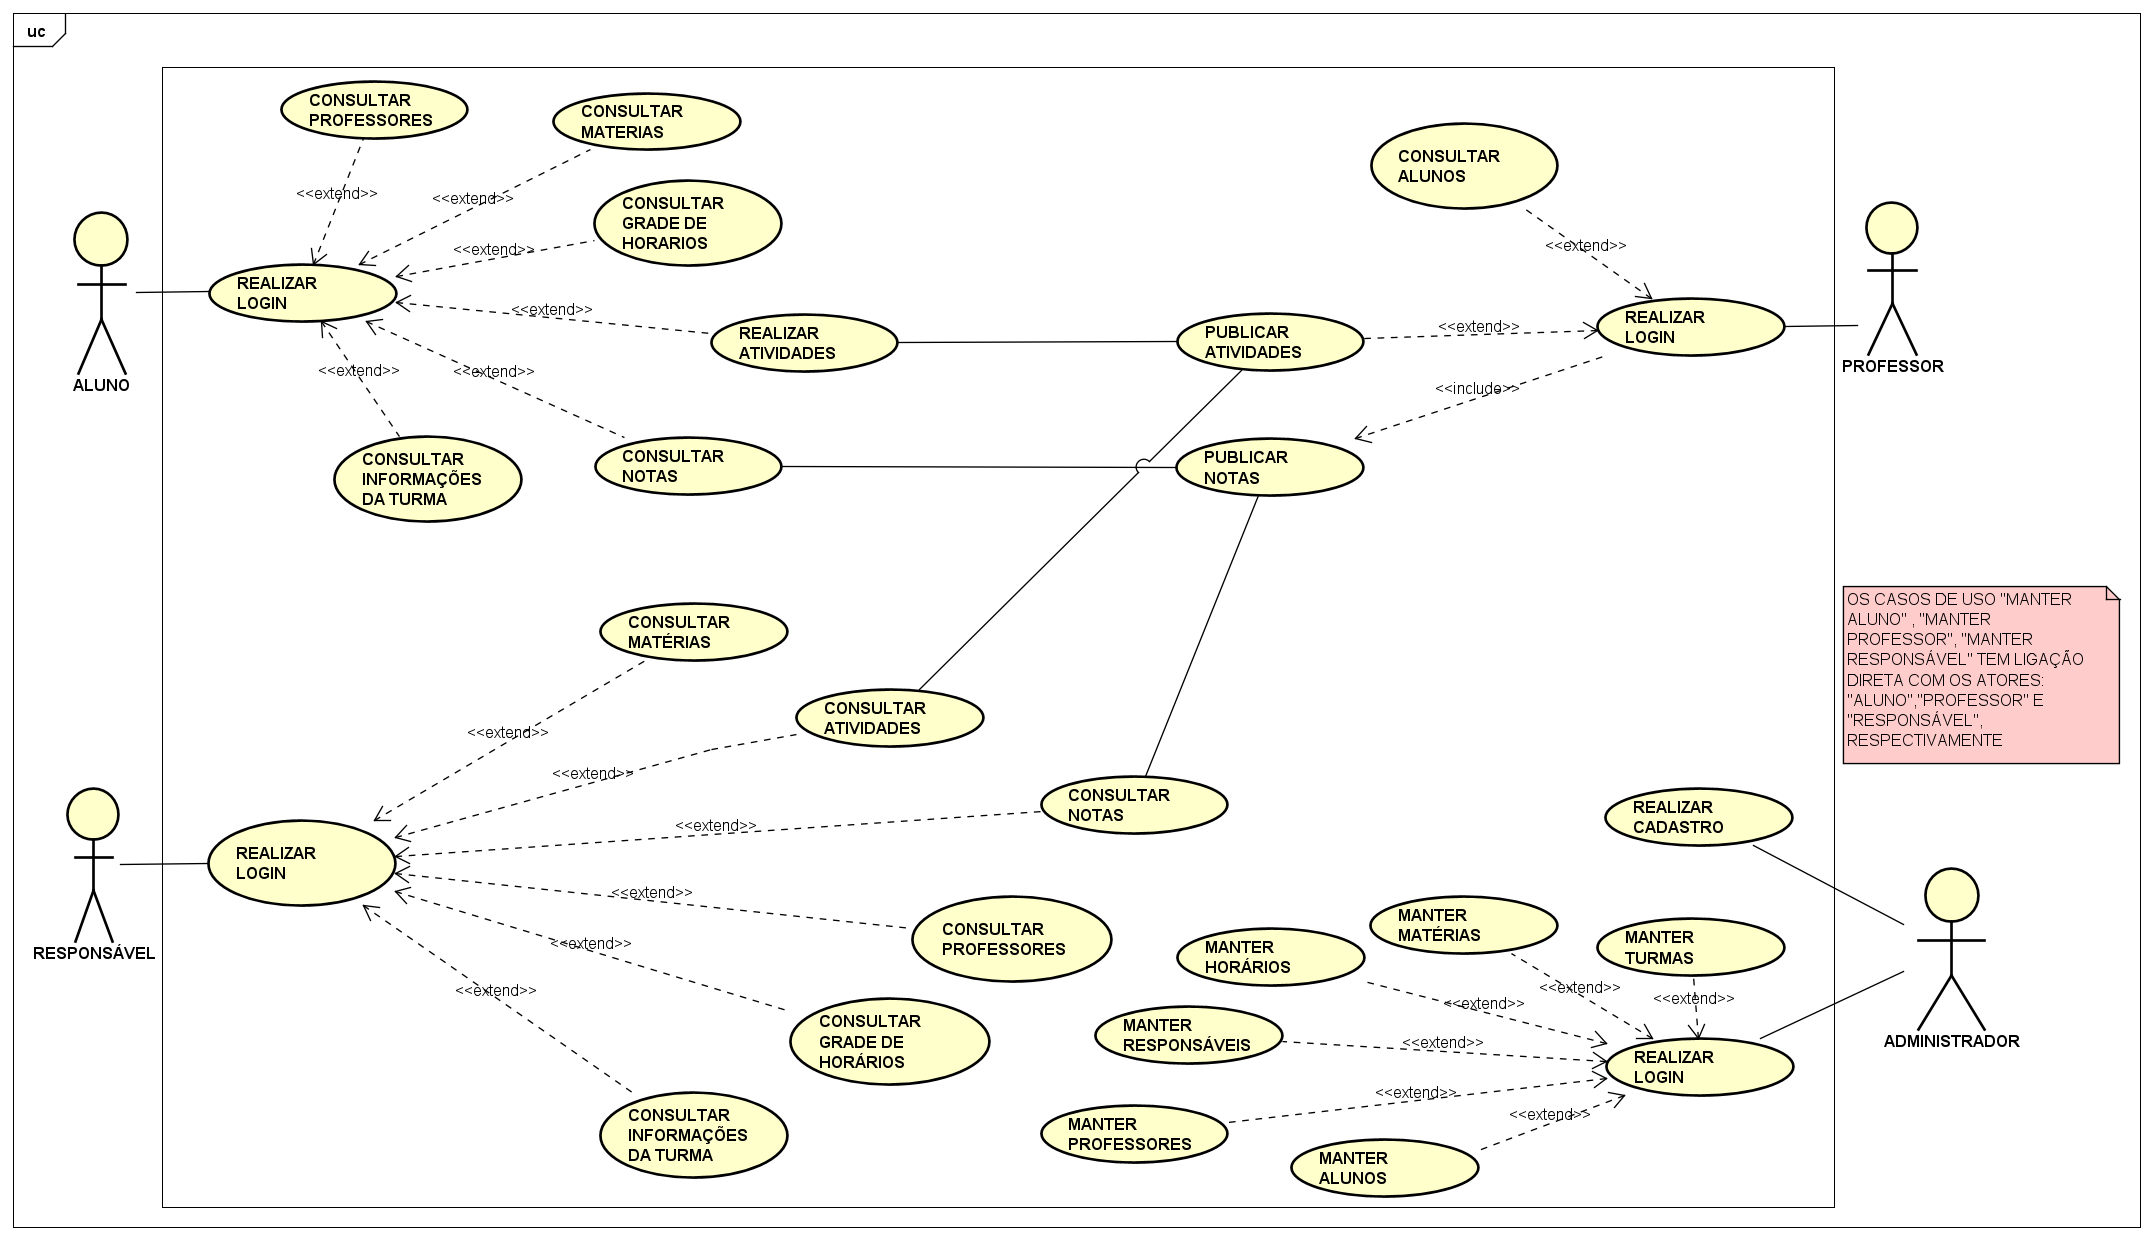
\includegraphics[scale=0.4, angle=-90]{dcu/dcu_geral}
    \caption{DCU Geral}
\end{figure}
% -------------------------------------------------------------------------------

% -------------------------------------------------------------------------------
\section{Desktop}

\subsection{Diagrama de Caso de Uso Desktop}
\begin{figure}[H]
    \centering
    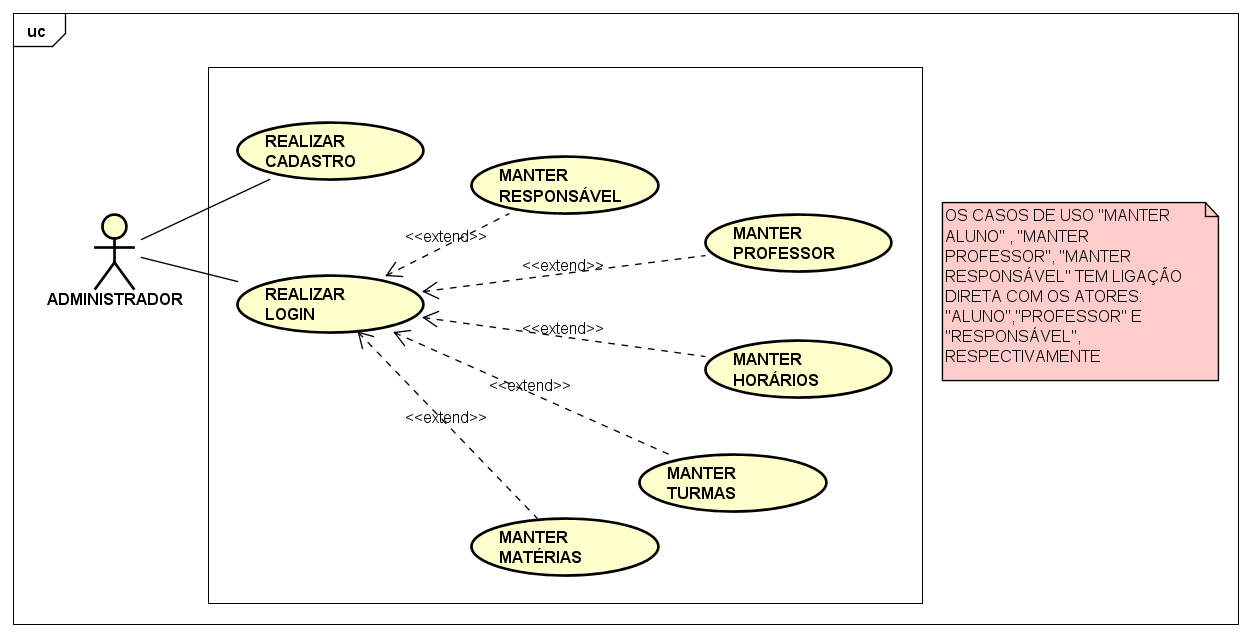
\includegraphics[scale=0.67, angle=-90]{dcu/dcu_adm}
    \caption{DCU Desktop}
\end{figure}

\includepdf[pages=-, pagecommand={\thispagestyle{fancy}}]{pdfs/cdu_desktop.pdf}
%\includepdf[pages=-]{pdfs/cdu_adm.pdf}

\subsection{Capturas de Tela Desktop}
Segue um excerto das páginas presentes no ambiente web, capturadas com o usuário ''Administrador'' logado no sistema.

\begin{figure}[H]
    \centering
    \hspace*{-0.7cm} % Ajuste o valor para mover a imagem para a esquerda
    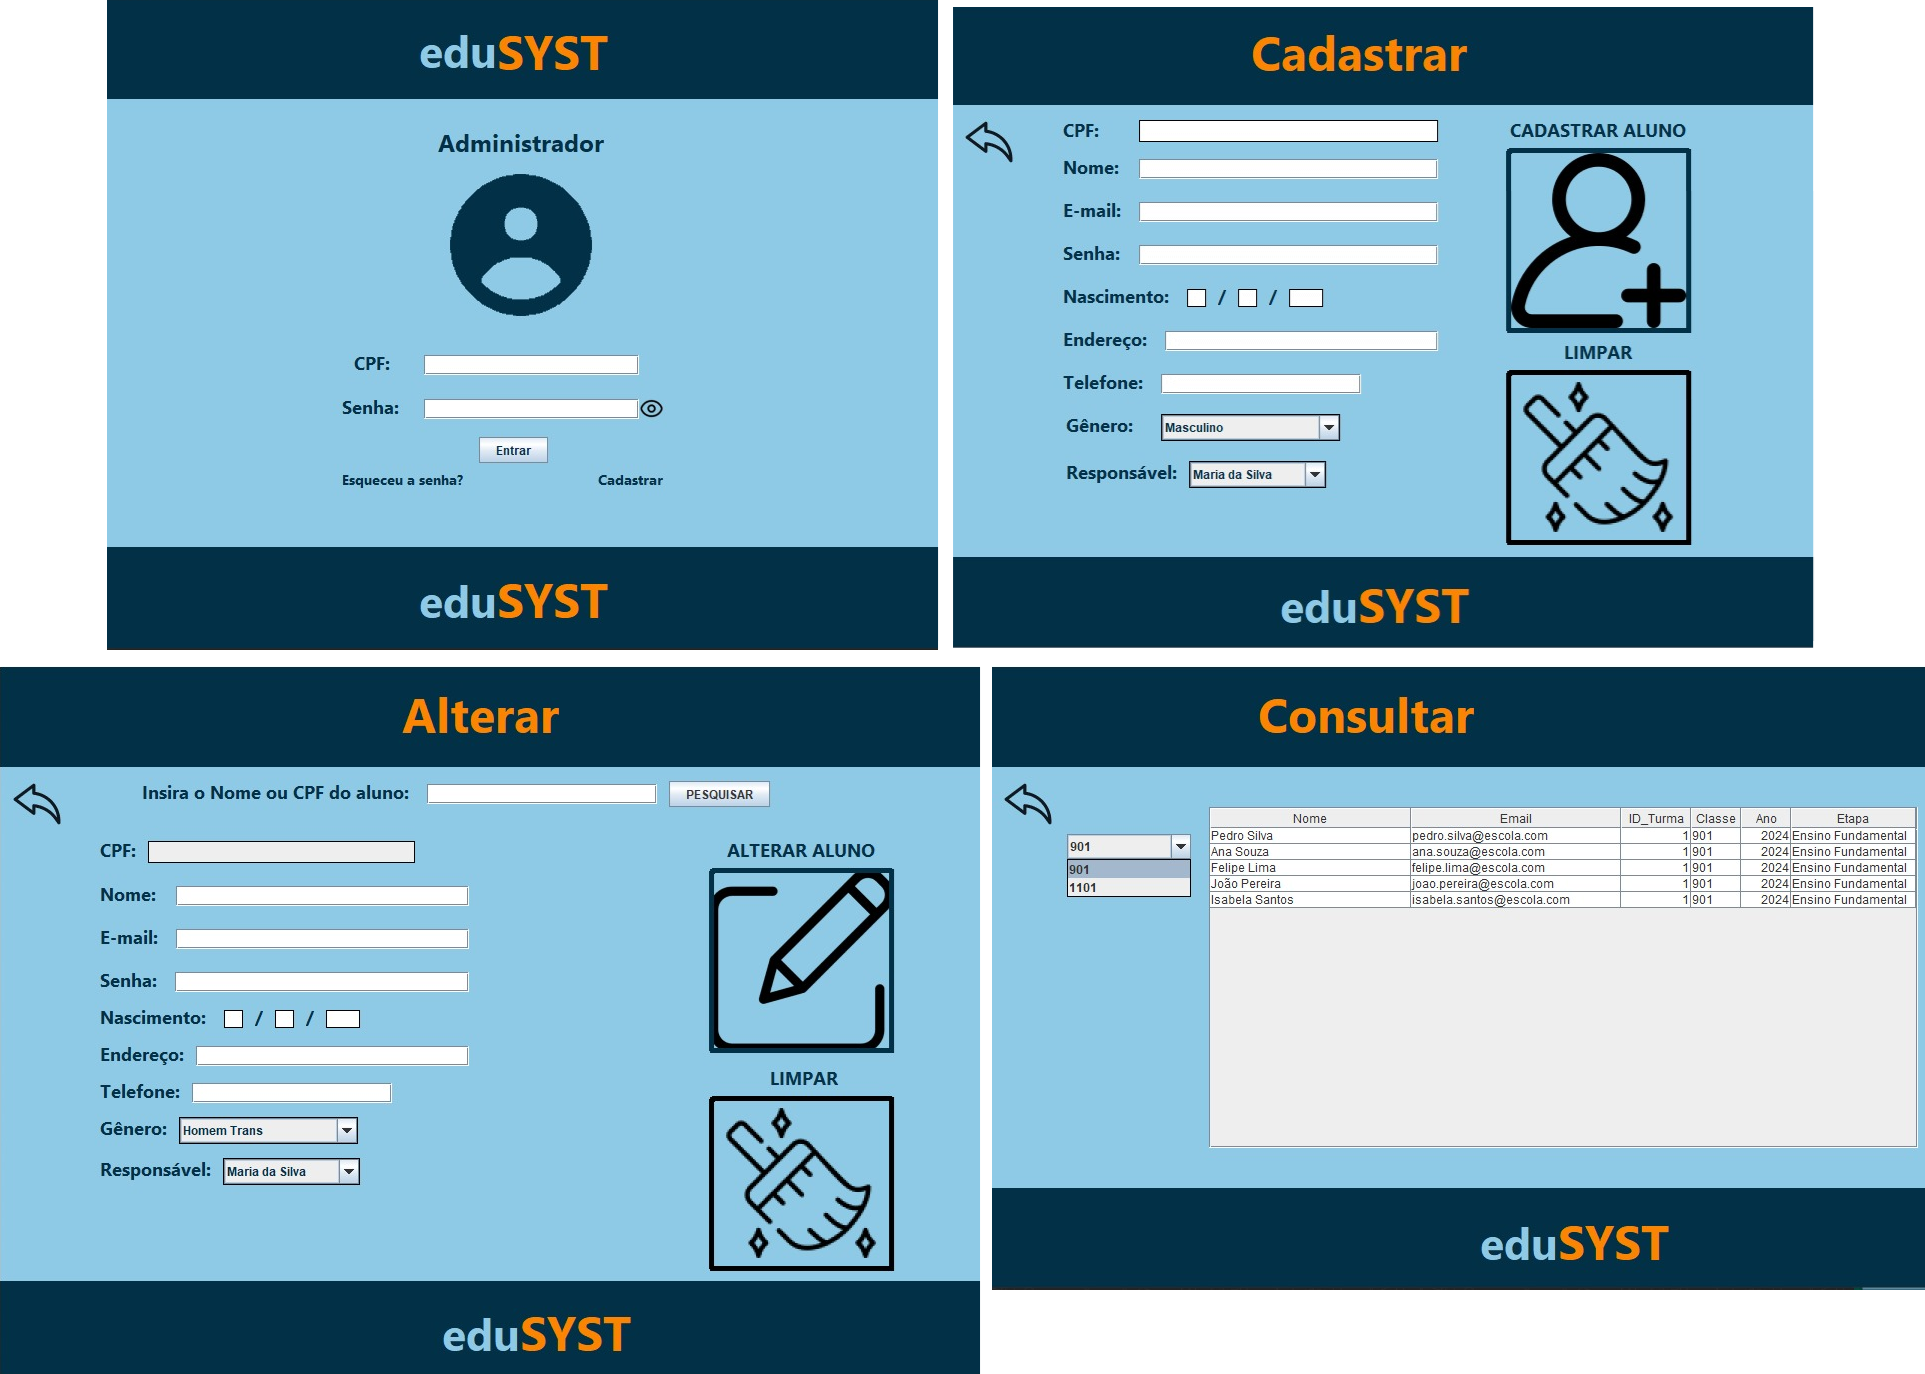
\includegraphics[scale=0.41, angle=-90]{scrshots/grade1_desk}
    \centering
    \caption{Telas - Login, Cadastro e Alteração de Alunos e Consulta de Turmas}
\end{figure}

\begin{figure}[H]
    \centering
    \hspace*{-0.7cm} % Ajuste o valor para mover a imagem para a esquerda
    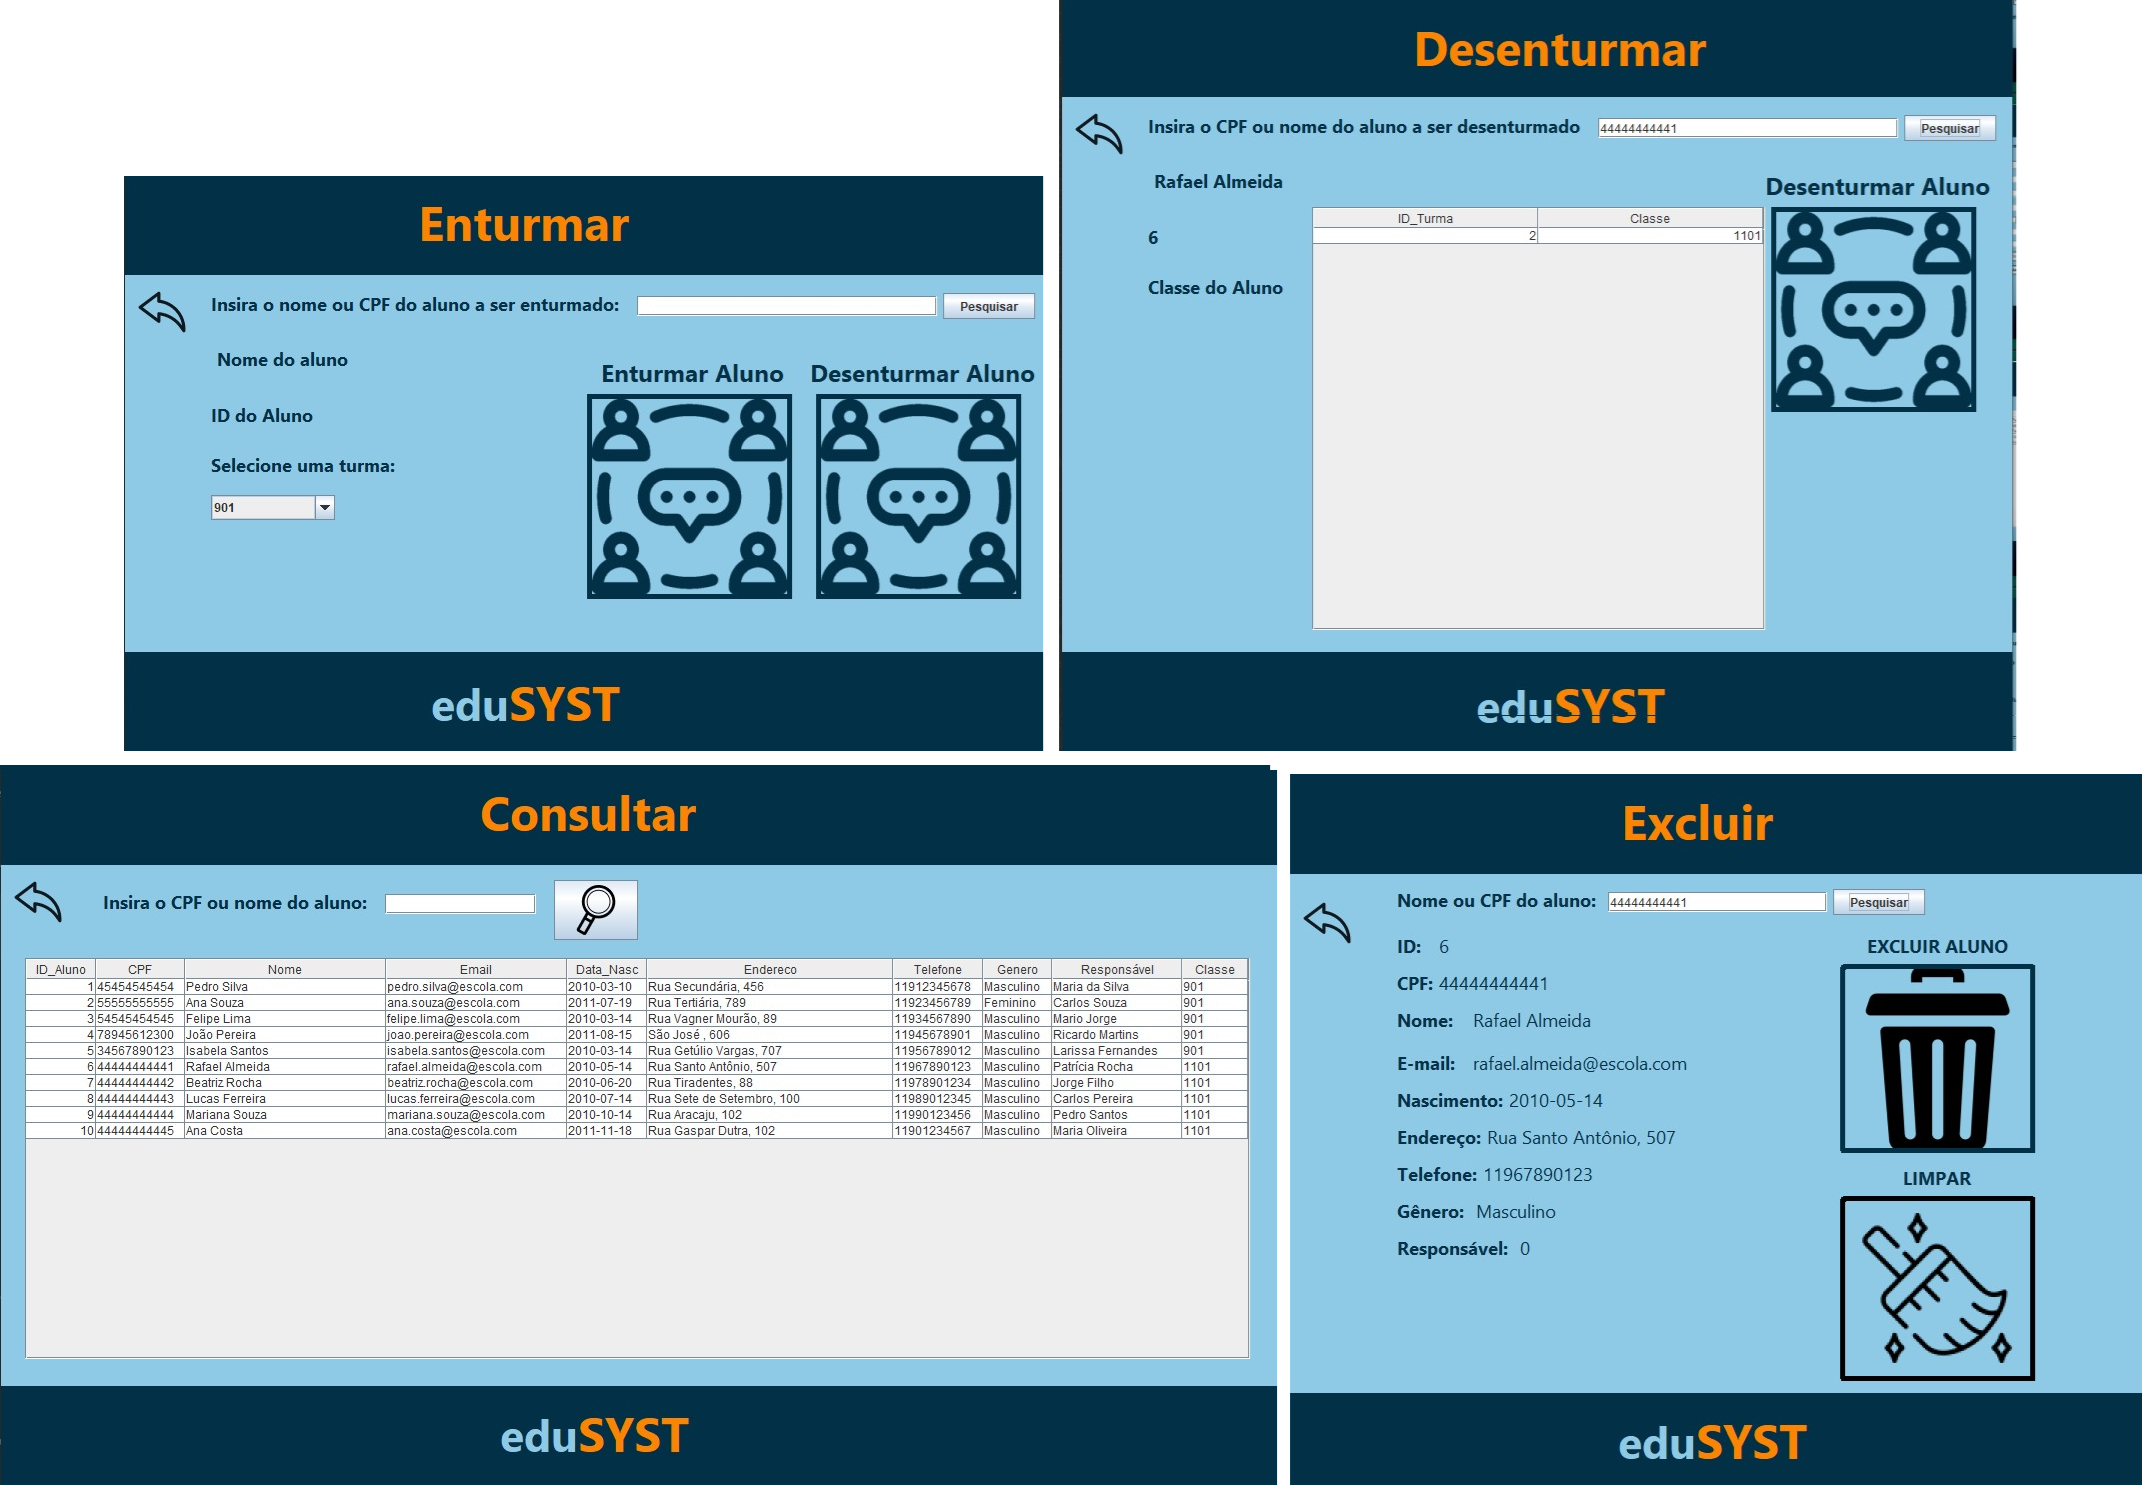
\includegraphics[scale=0.41, angle=-90]{scrshots/grade2_desk}
    \centering
    \caption{Telas - Enturmação, Desenturmação, Consulta e Exclusão de Alunos}
\end{figure}
% -------------------------------------------------------------------------------

% -------------------------------------------------------------------------------
\section{Web}

\subsection{Diagrama de Caso de Uso Web}
\begin{figure}[H]
    \centering
    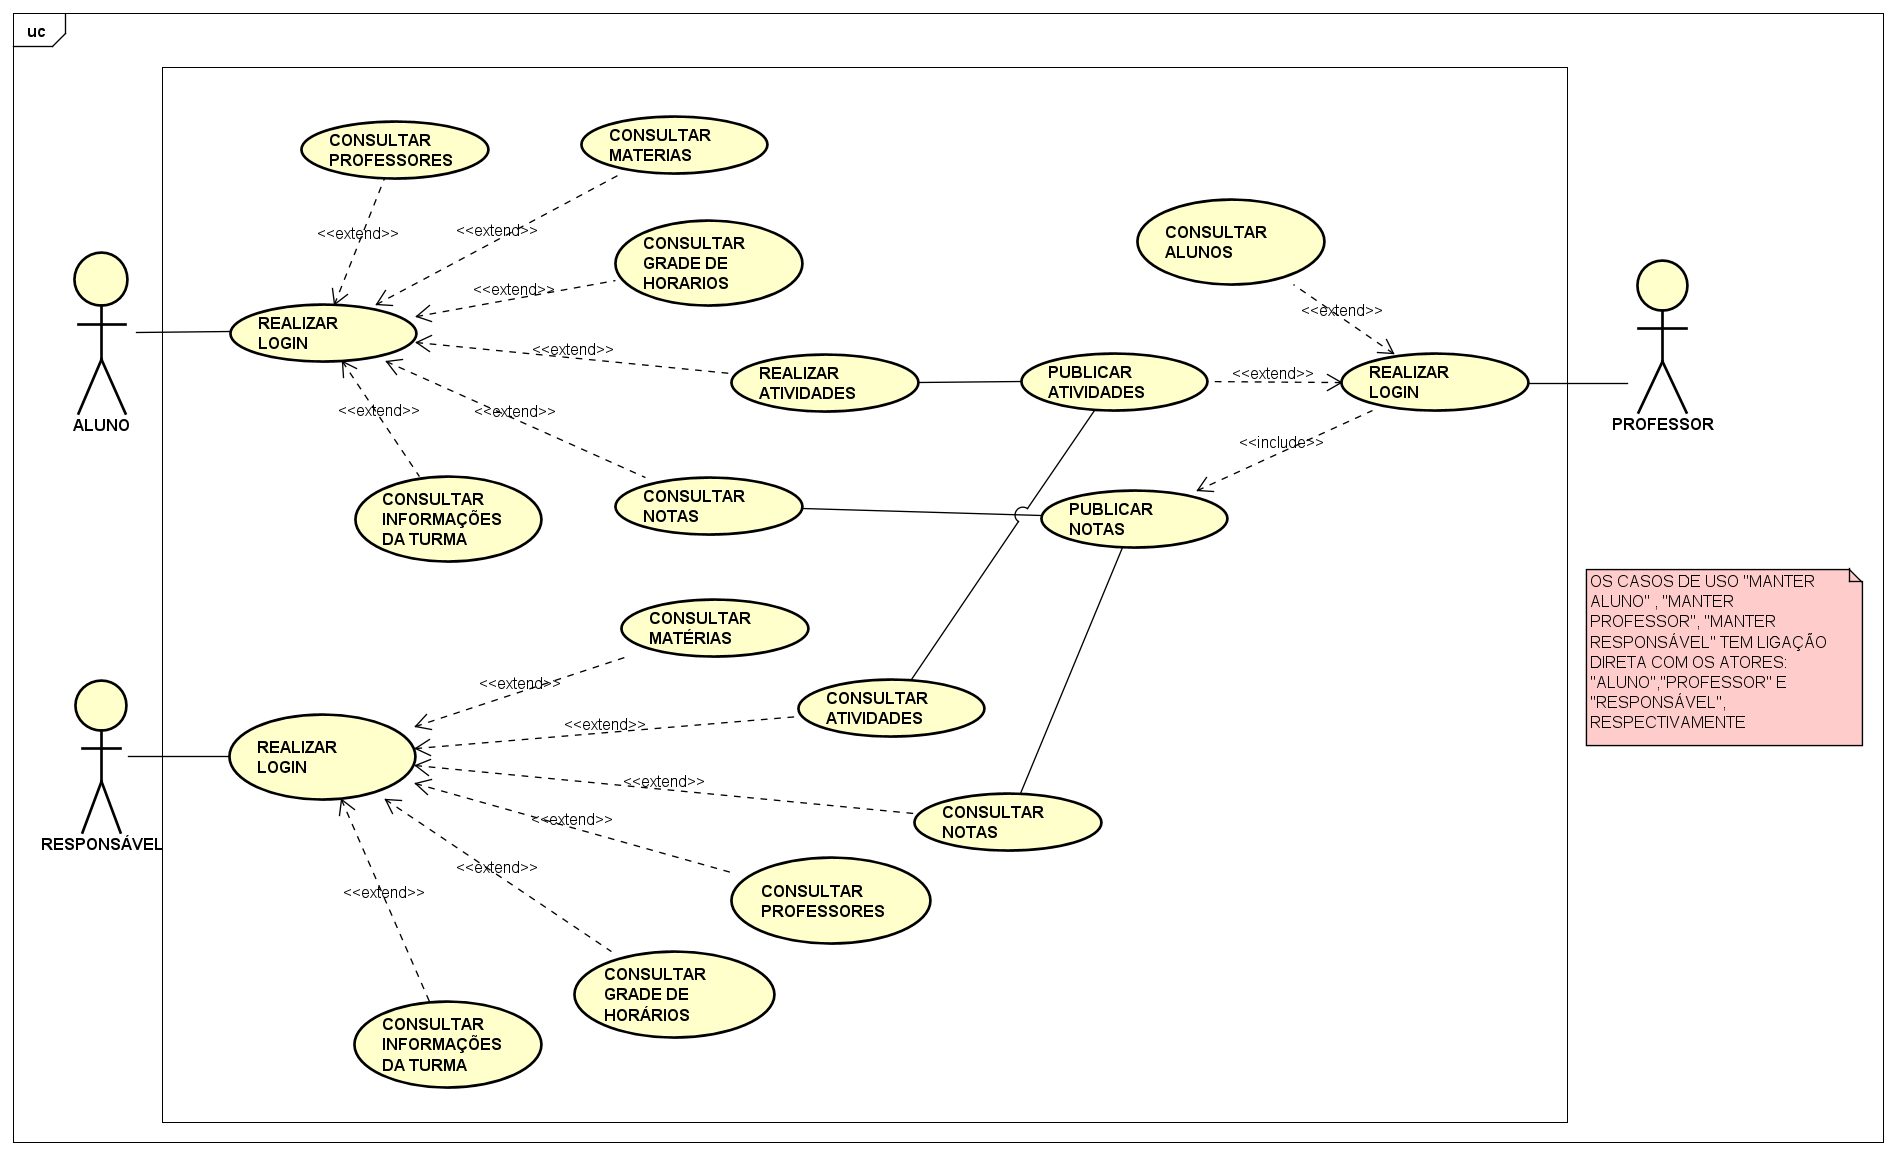
\includegraphics[scale=0.44, angle=-90]{dcu/dcu_web}
    \caption{DCU WEB}
\end{figure}

\includepdf[pages=-, pagecommand={\thispagestyle{fancy}}]{pdfs/cdu_web.pdf}
%\includepdf[pages=-]{pdfs/cdu_web.pdf}

\subsection{Capturas de Tela Web}
Segue um excerto das páginas presentes no ambiente web, capturadas com o usuário ''Professor'' logado no sistema.

\begin{figure}[H]
    \centering
    \hspace*{-0.7cm} % Ajuste o valor para mover a imagem para a esquerda
    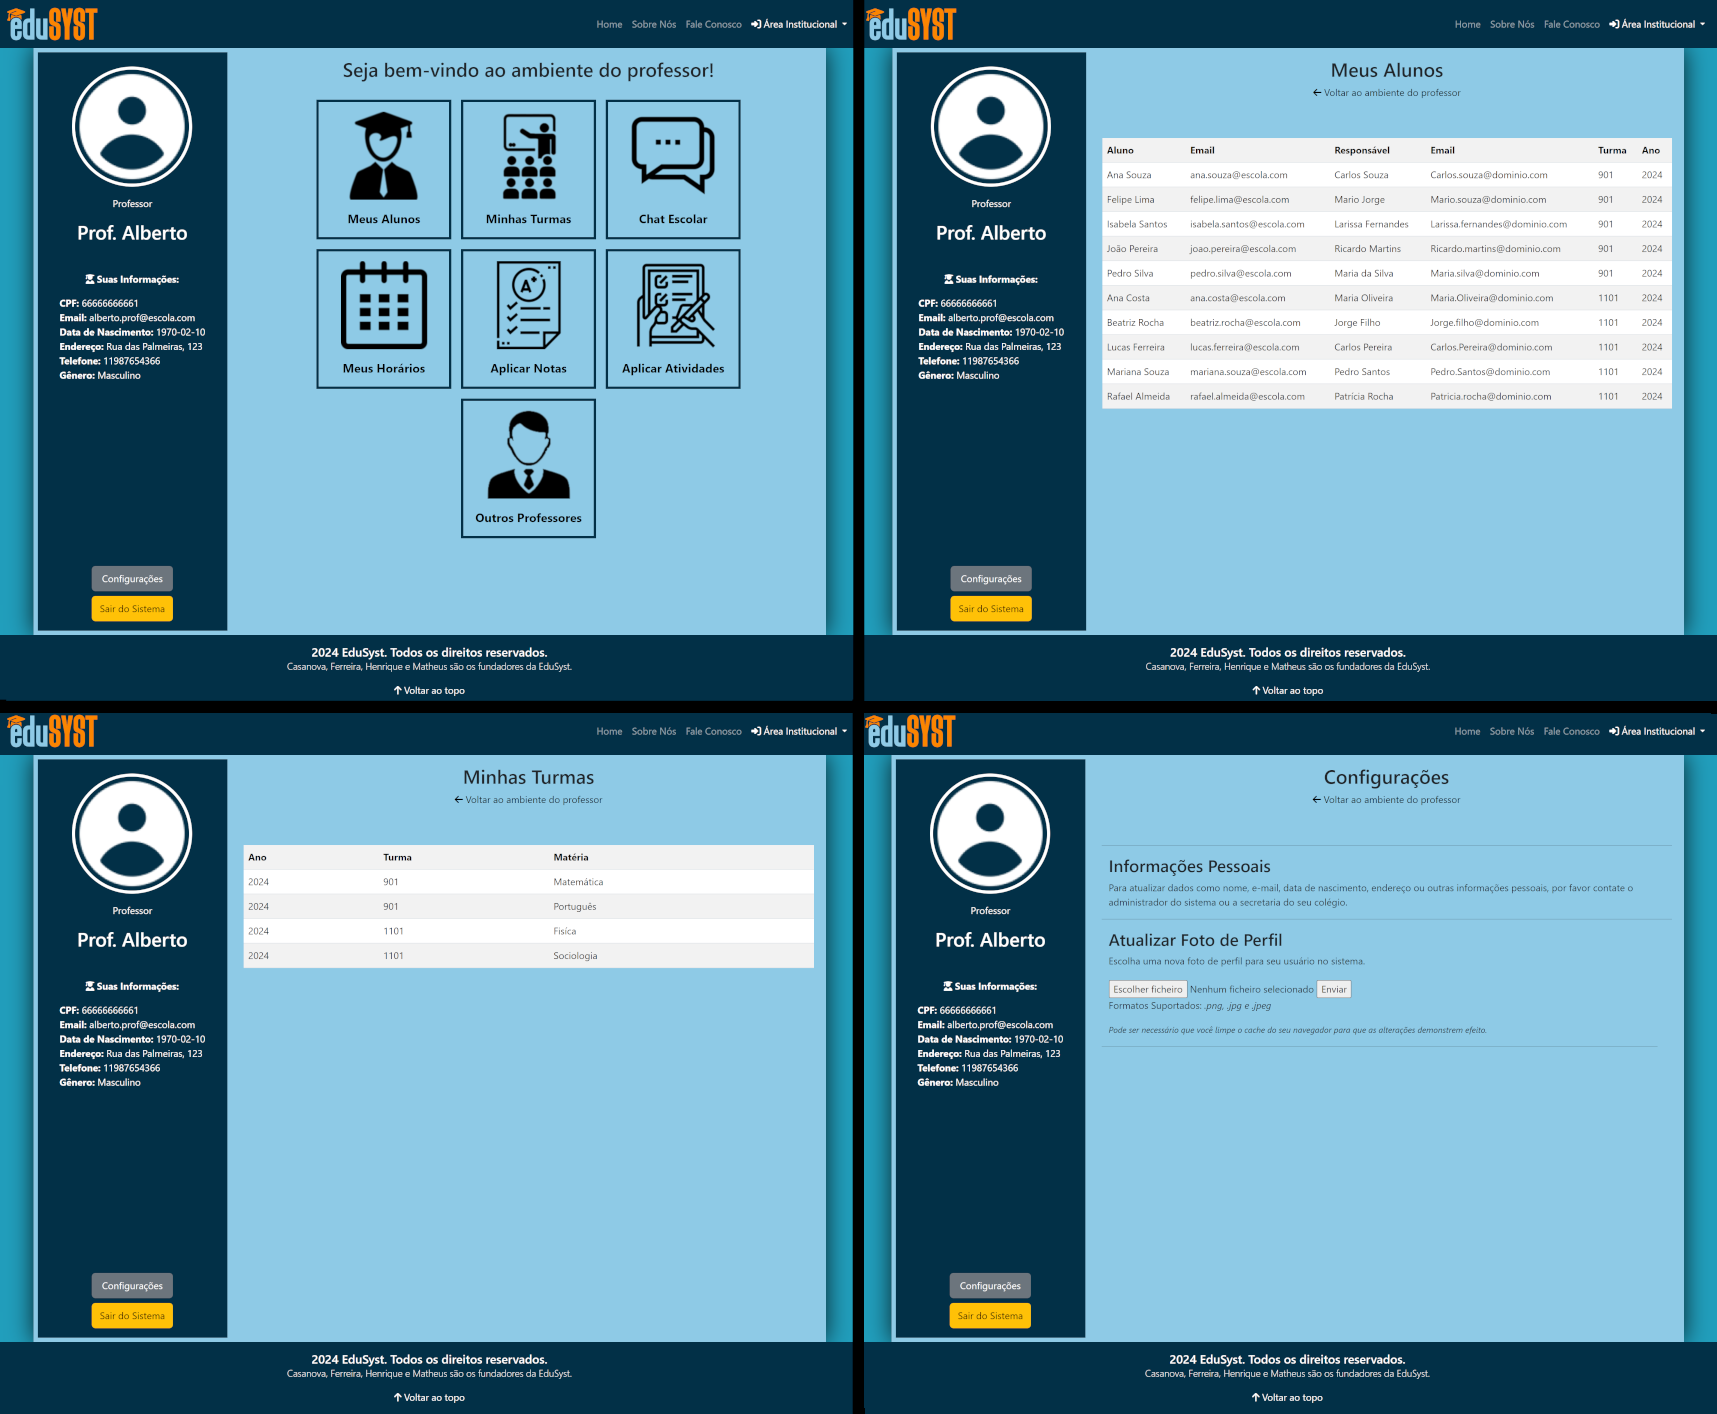
\includegraphics[scale=0.34, angle=-90]{scrshots/grade2}
    \centering
    \caption{Páginas - Página de usuário, Alunos, Turmas e Configurações do Perfil}
\end{figure}
\begin{figure}[H]
    \centering
    \hspace*{-0.7cm} % Ajuste o valor para mover a imagem para a esquerda
    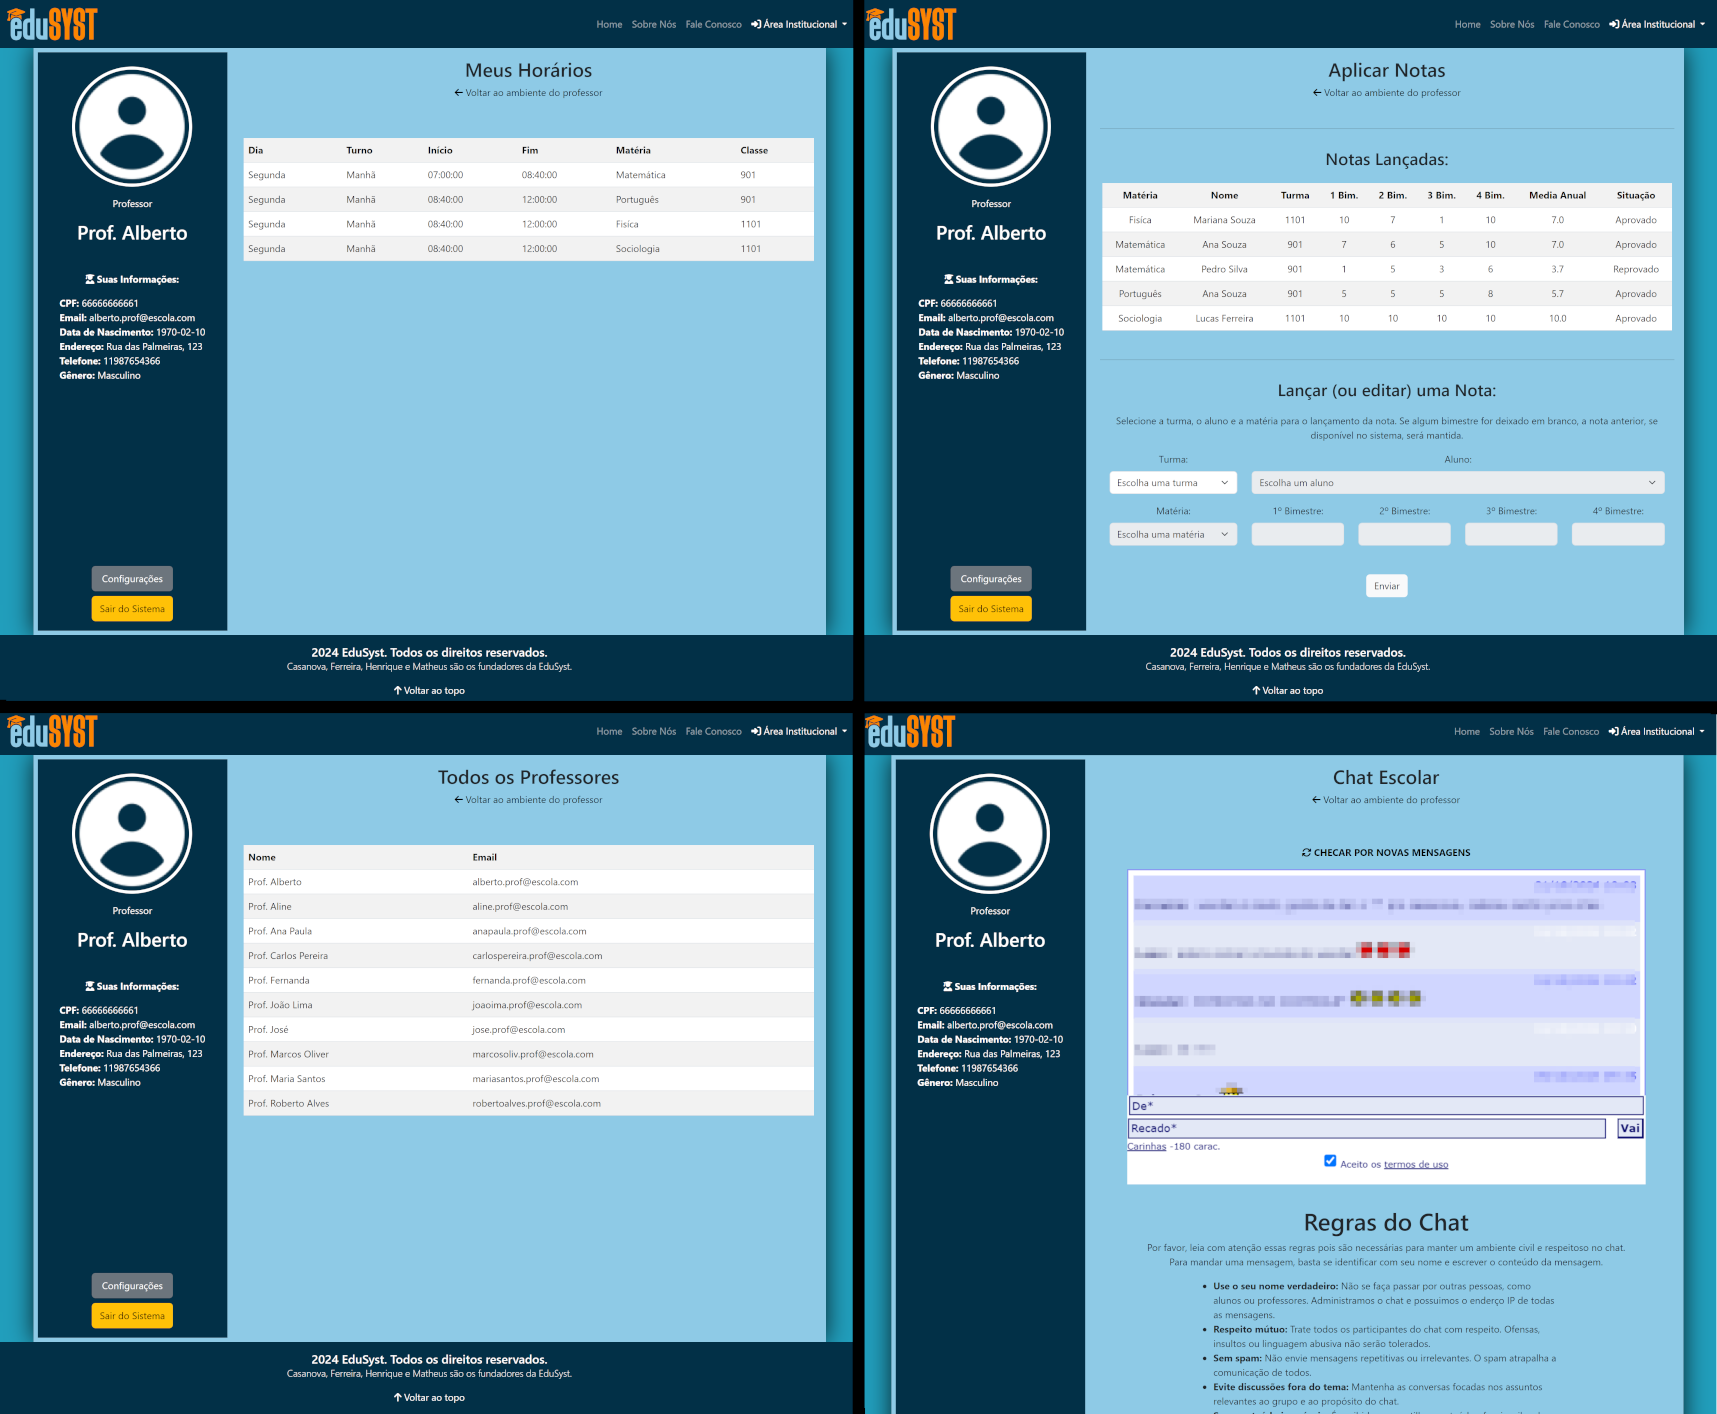
\includegraphics[scale=0.34, angle=-90]{scrshots/grade1}
    \caption{Páginas - Grade de Horários, Aplicação de Notas, Listagem de Professores e Chat}
\end{figure}

% \subsection{Fluxo de Páginas Web} % NÃO SEI SE VAI TER!
% -------------------------------------------------------------------------------

% -------------------------------------------------------------------------------
\section{Android}

\subsection{Diagrama de Caso de Uso Android}
\begin{figure}[H]
    \centering
    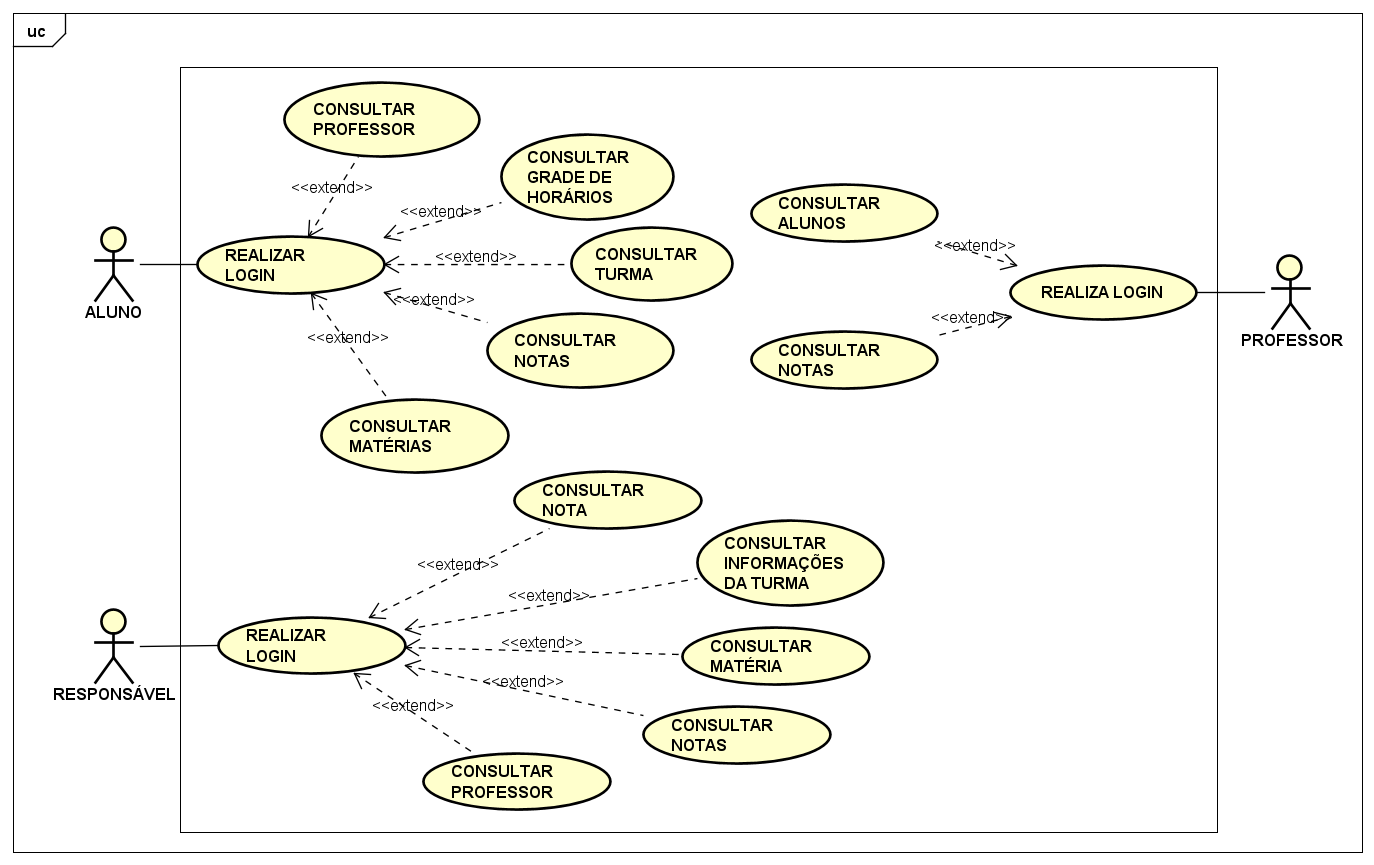
\includegraphics[scale=0.58, angle=-90]{dcu/dcu_android}
    \caption{DCU Android}
\end{figure}

\subsection{Descrição do Sistema ``EduSYST'' Android}
A funcionalidade do sistema Android é idêntica a funcionalidade do sistema WEB, com exceção dos seguintes casos de uso indisponíveis no sistema Android:

\begin{itemize}
    \item Ator: Aluno
    \begin{enumerate}
        \item Não é possível realizar atividades. (CdU-9 do ator Aluno)
    \end{enumerate}

    \item Ator: Responsável
    \begin{enumerate}
        \item Não é possível consultar atividades do aluno associado ao responsável. (CdU-16 do ator Responsável)
    \end{enumerate}

    \item Ator: Professor
    \begin{enumerate}
        \item Não é possível publicar atividades. (CdU-18 do ator Professor)
        \item Não é possível publicar notas. (CdU-19 do ator Professor)
    \end{enumerate}
\end{itemize}

\newpage
\subsection{Capturas de Tela Android}
Segue um excerto das telas presentes no aplicativo Android, capturadas com o usuário ''Aluno'' logado no sistema.
\begin{figure}[H]
    \centering
    \hspace*{-1.1cm} % Ajuste o valor para mover a imagem para a esquerda
    \centering
    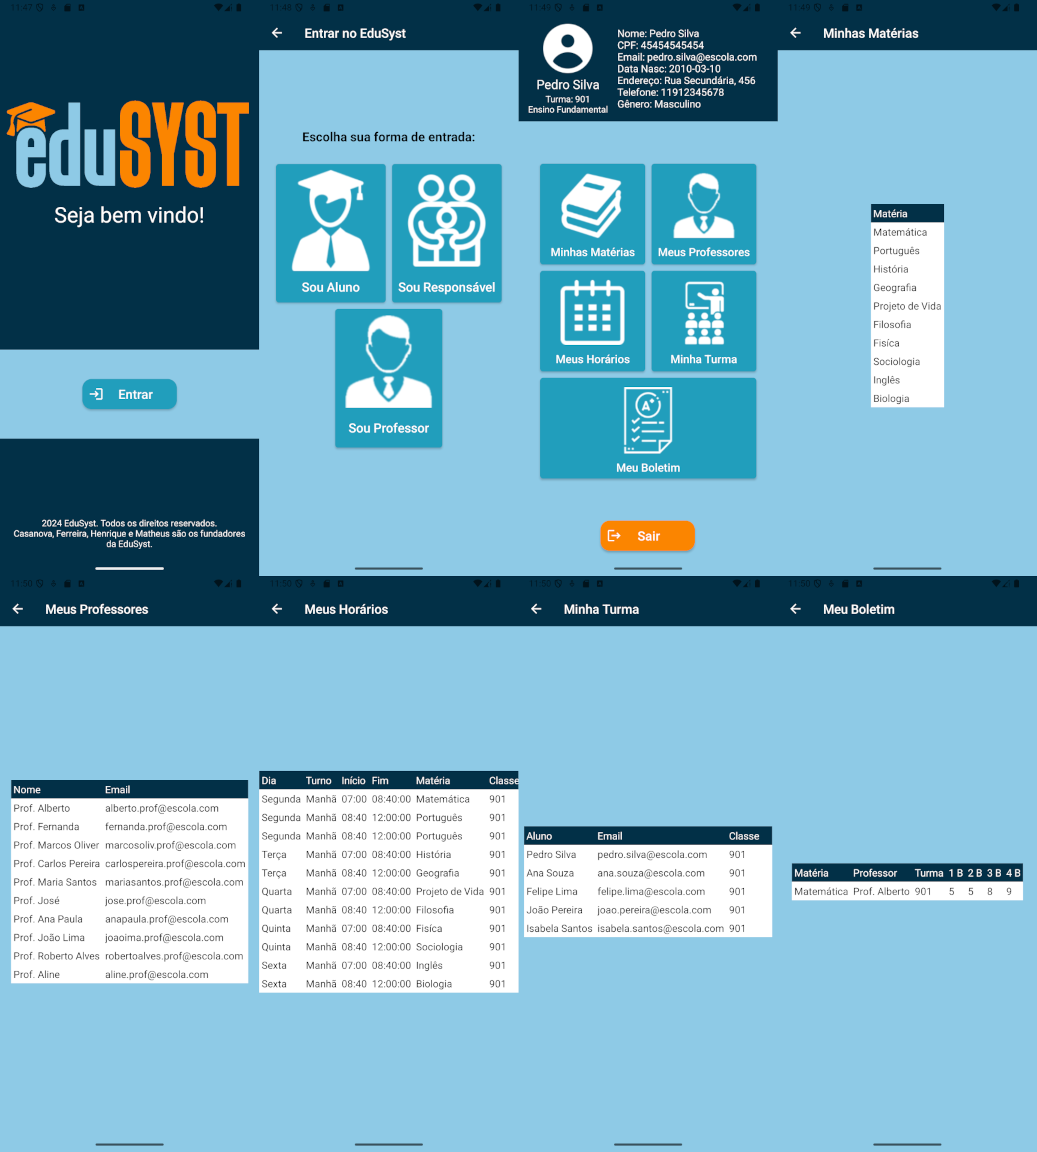
\includegraphics[scale=0.43, angle=-90]{scrshots/grade1_and}
    \caption{Telas - Login, Opções, Matérias, Professores, Horários, Turma e Boletim}
\end{figure}

% \subsection{Fluxo de Páginas Android} % NÃO SEI SE VAI TER!
% -------------------------------------------------------------------------------

% -------------------------------------------------------------------------------
\section{Banco de Dados}

\subsection{Diagrama de Entidade-Relacionamento}
\begin{figure}[H]
    \centering
    \hspace*{-1.1cm} % Ajuste o valor para mover a imagem para a esquerda
    \centering
    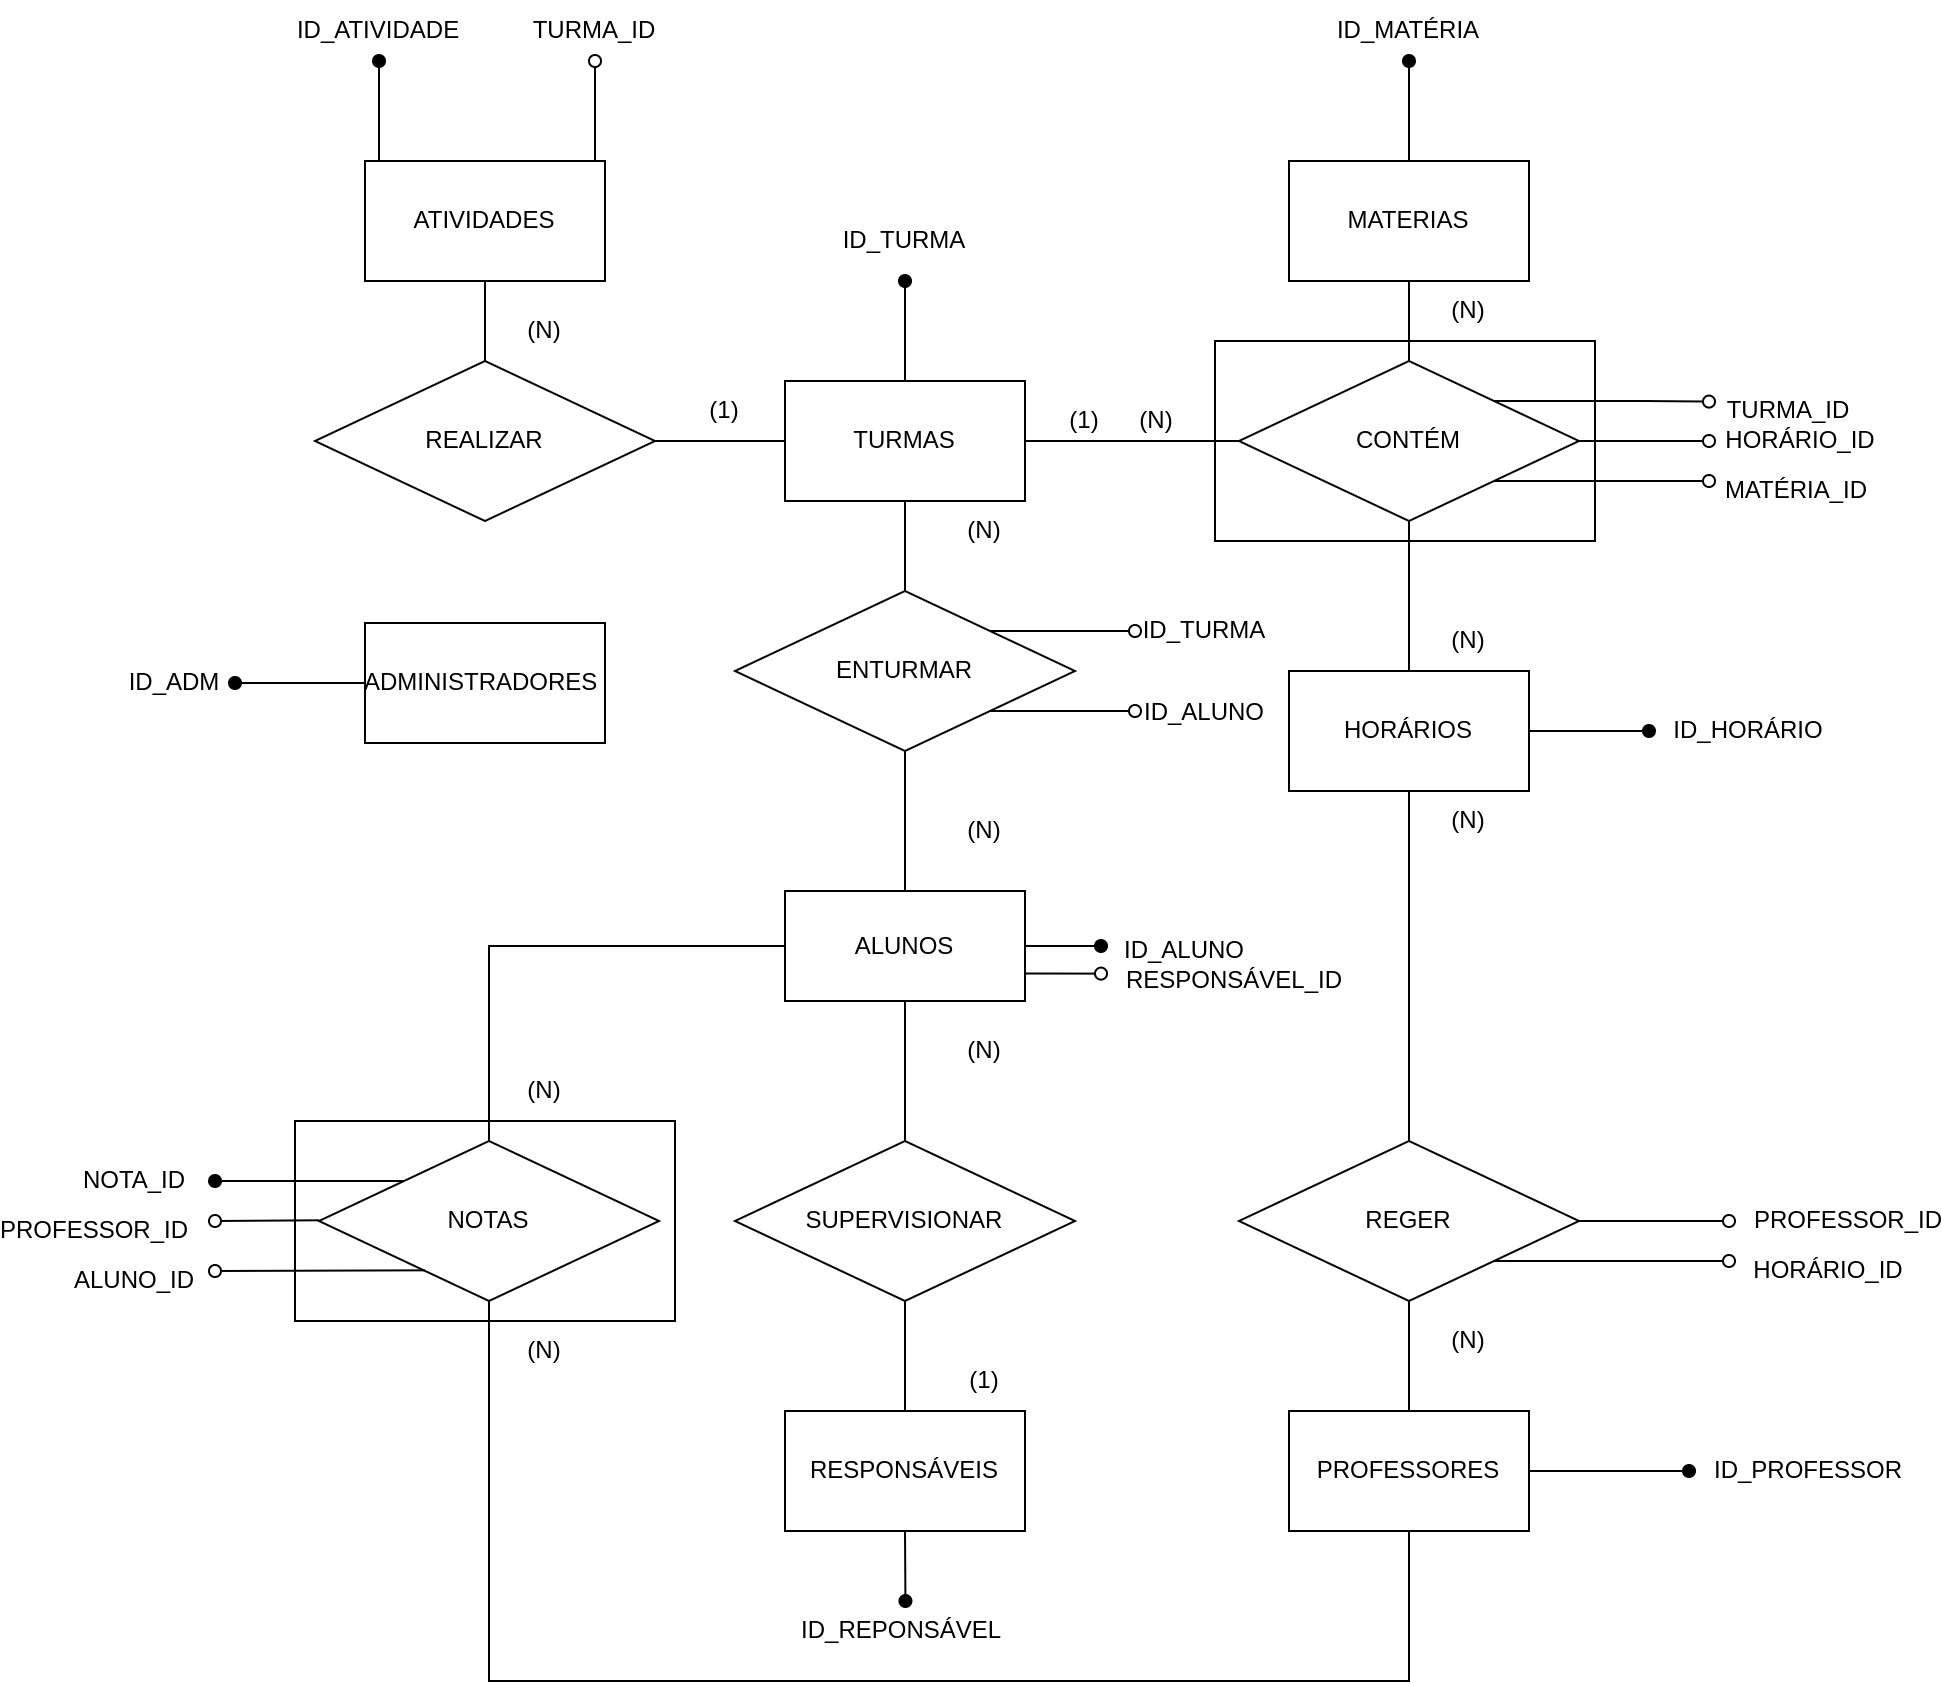
\includegraphics[scale=0.29, angle=-90]{der}
    \caption{DER}
\end{figure}

\subsection{Diagrama Lógico}
\begin{figure}[H]
    \centering
    \hspace*{-1.3cm} % Ajuste o valor para mover a imagem para a esquerda
    \centering
    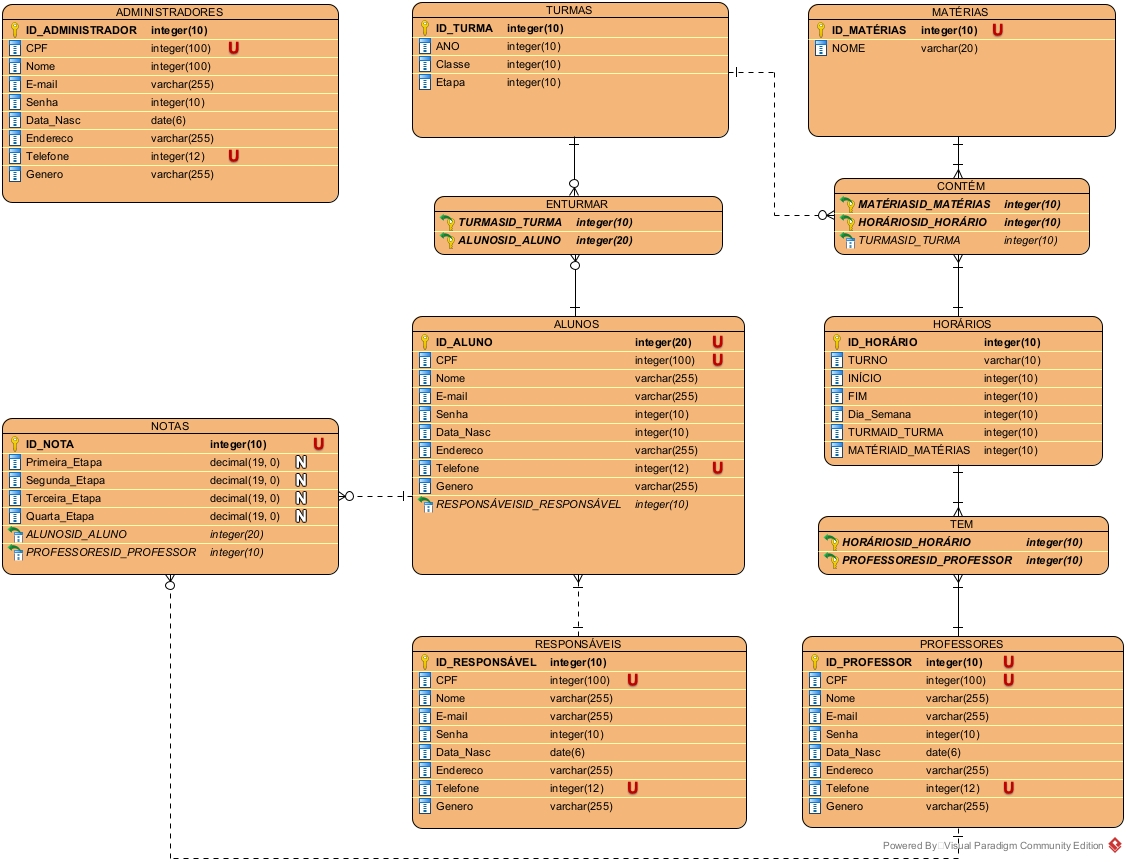
\includegraphics[scale=0.55, angle=-90]{dclas}
    \caption{Diagrama Lógico}
\end{figure}

\subsection{Diagrama de Classes}
\begin{figure}[H]
    \centering
    \vspace*{-0.5cm} % Ajuste o valor para mover a imagem para a 
    \hspace*{-2.72cm} % Ajuste o valor para mover a imagem para a esquerda
    \centering
    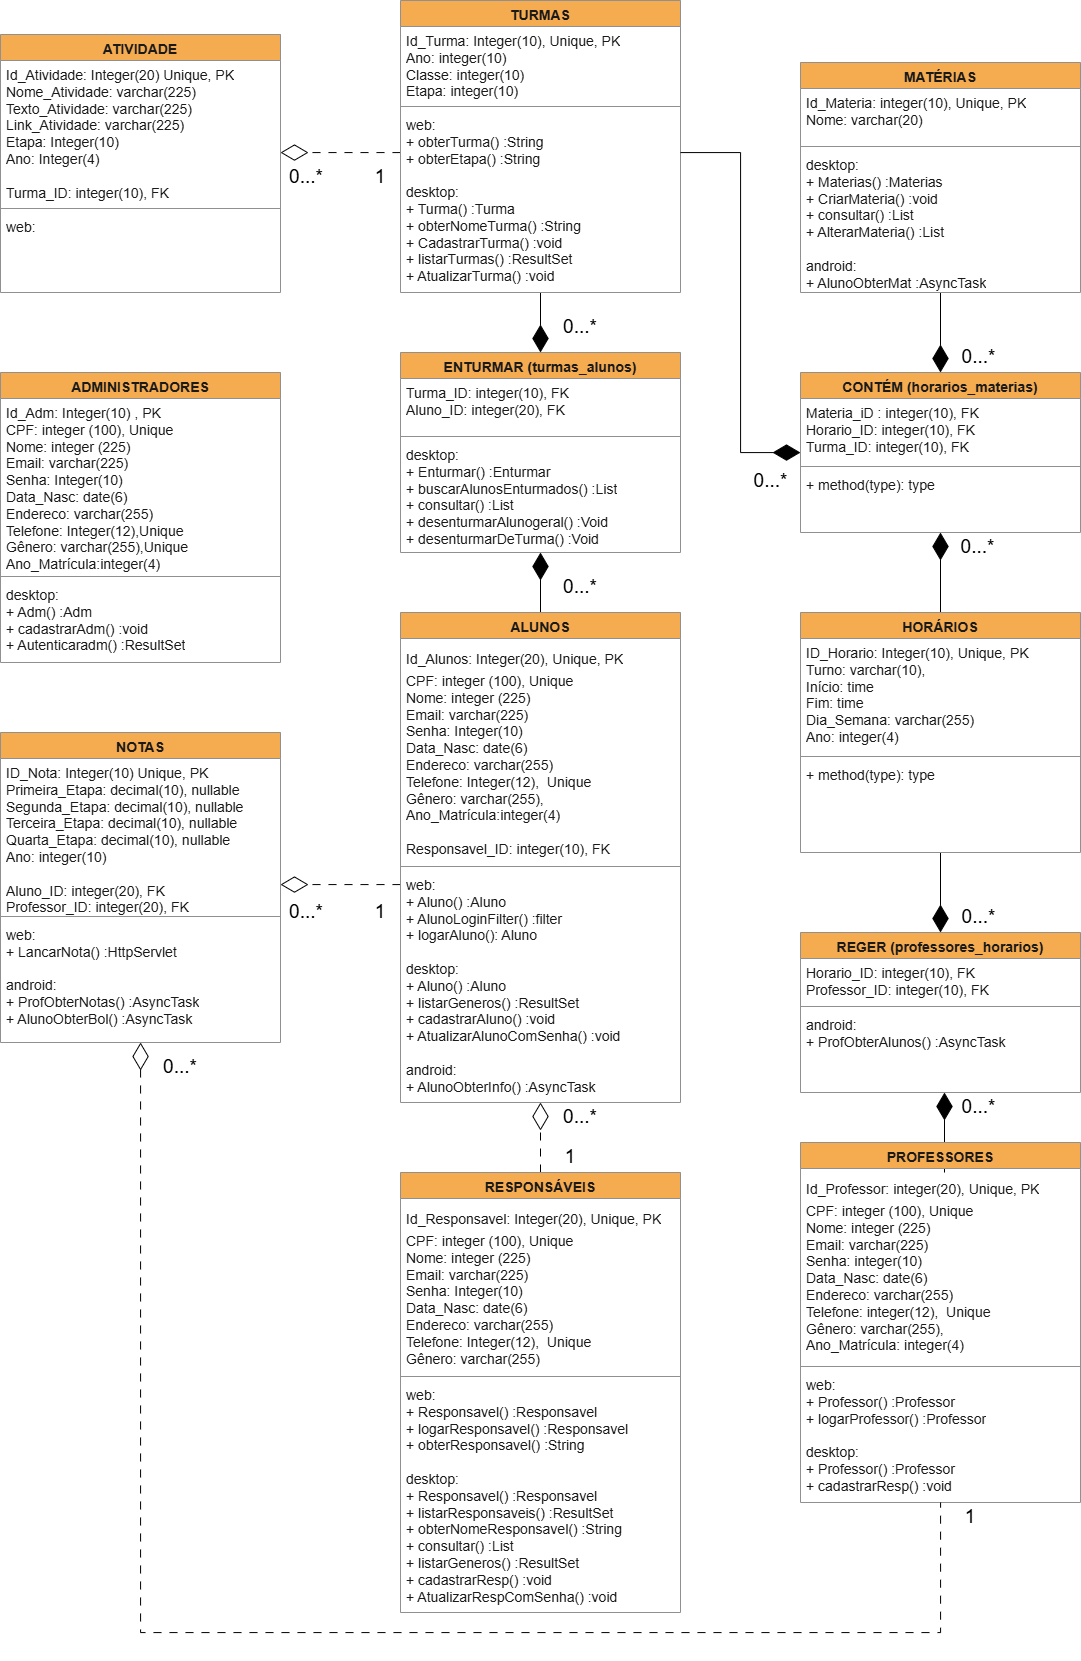
\includegraphics[width=1.27\textwidth, height=1.61\textwidth, angle=0]{dclas2}
    \caption{Diagrama de Classes}
\end{figure}

\subsection{Observações Sobre a Entidade Notas}
A tabela Notas no banco de dados do EduSyst estabelece relacionamentos entre os Alunos e os Professores. Embora à primeira vista esses relacionamentos possam parecer circulares, na verdade eles são relacionamentos unidirecionais que seguem uma estrutura hierárquica clara, sem a formação de laços circulares.

Na estrutura, cada nota depende exclusivamente de duas entidades principais: o Aluno que a recebe e o Professor que a atribui. A chave estrangeira Aluno\underline{\hspace{.10in}}ID conecta a tabela de Notas à tabela de Alunos, e a chave Professor\underline{\hspace{.10in}}ID faz o vínculo com a tabela de Professores. No entanto, esses relacionamentos não são circulares, pois a definição de uma nota não retroalimenta nenhum dos dois lados — os dados de notas fluem unicamente do aluno e do professor para a tabela de Notas.

Em termos práticos, uma relação circular seria se os dados tivessem que voltar ao ponto de origem em um ciclo contínuo, ou se houvesse dependência cíclica para resolver as informações de maneira infinita. No caso da tabela Notas, o relacionamento segue uma hierarquia linear: os professores atribuem notas aos alunos, e essas notas são armazenadas como registros específicos de cada aluno-professor na tabela Notas. Não há necessidade de uma entidade depender do retorno de outra para completar o ciclo.

\subsection{Backup e Particionamento dos Dados}
O sistema de backup e armazenamento de dados implementado no banco de dados do EduSyst visa garantir a integridade e preservação das informações dos usuários. Para isso, são utilizadas tabelas “mortas” não representadas no diagrama de classes (TM\_Responsaveis, TM\_Alunos e TM\_Professores), que atuam como repositórios de backup particionados para os dados de usuários, sendo cada tabela configurada com cinco partições proporcionais, definidas pela chave primária dos usuários. As tabelas de backup replicam as estruturas principais e contêm os campos relevantes, como CPF, Nome, Email e outros atributos específicos de cada entidade.

Para garantir que qualquer novo dado seja automaticamente registrado nas tabelas de backup, foram criadas procedures triggers (disparadores) que executam ações após a inserção de registros nas tabelas respectivas. Cada trigger — BackupResponsaveis, BackupAlunos e BackupProfessores — é programado para, após um INSERT, inserir uma cópia exata dos dados nas respectivas tabelas mortas. Assim, é possível manter um histórico de docentes e alunos, fazer seleções de forma mais prática (graça às partições) e facilitando a recuperação de dados, caso haja necessidade.

\subsection{Amostragem de Dados Fictícios}
Segue um excerto das informações fictícias contidas no banco de dados por padrão, disponíveis no momento de sua criação.

% \subsection{Dados da Tabela ``Administradores''}
\begin{figure}[H]
    \centering
    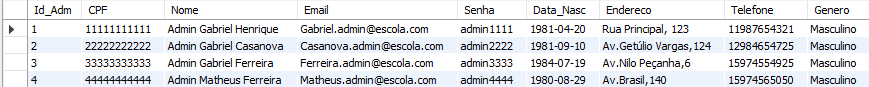
\includegraphics[scale=0.65]{tabelas/tabela_adm}
    \caption{Tabela Administradores}
\end{figure}
%\subsection{Tabela ``Responsáveis''}
\begin{figure}[H]
    \centering
    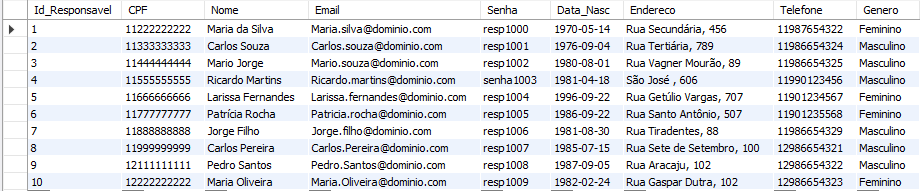
\includegraphics[scale=0.65]{tabelas/tabela_resp}
    \caption{Tabela Responsáveis}
\end{figure}
%\subsection{Tabela ``Alunos''}
\begin{figure}[H]
    \centering
    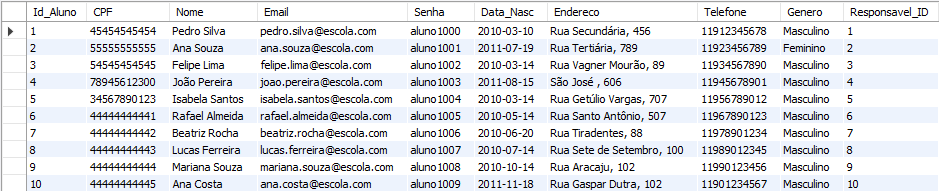
\includegraphics[scale=0.65]{tabelas/tabela_alunos}
    \caption{Tabela Alunos}
\end{figure}
%\subsection{Tabela ``Professores''}
\begin{figure}[H]
    \centering
    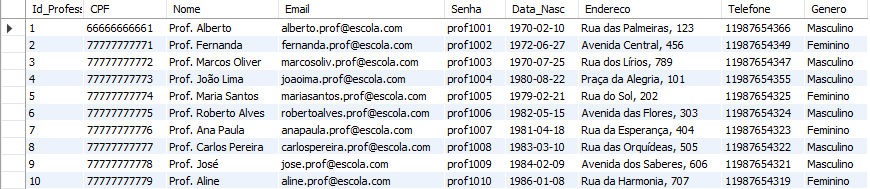
\includegraphics[scale=0.65]{tabelas/tabela_profs}
    \caption{Tabela Professores}
\end{figure}
\begin{figure}[H]
    \centering
    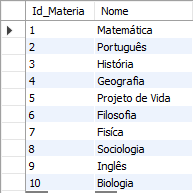
\includegraphics[scale=0.65]{tabelas/tabela_materias}
    \caption{Tabela Matérias}
\end{figure}
\begin{figure}[H]
    \centering
    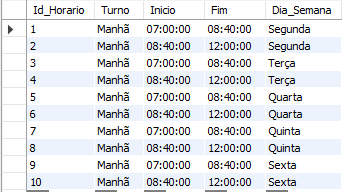
\includegraphics[scale=0.65]{tabelas/tabela_horarios}
    \caption{Tabela Horários}
\end{figure}

% -------------------------------------------------------------------------------

% -------------------------------------------------------------------------------
\section{Prints do Núcleo do Sistema}
A seguir, são apresentados trechos essenciais do código do sistema, destacando os métodos e classes fundamentais. Esse excerto não representa a totalidade do código, mas sim áreas notáveis de cada parte do sistema.

\subsection{Java Web / JSP}
\begin{figure}[H]
    \centering
    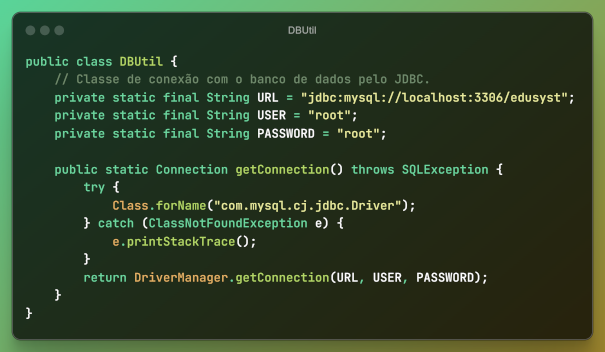
\includegraphics[scale=0.6]{imagens/code_scrs/2-db}
    \caption{Conexão com o Banco de Dados MySQL}
\end{figure}

\begin{figure}[H]
    \centering
    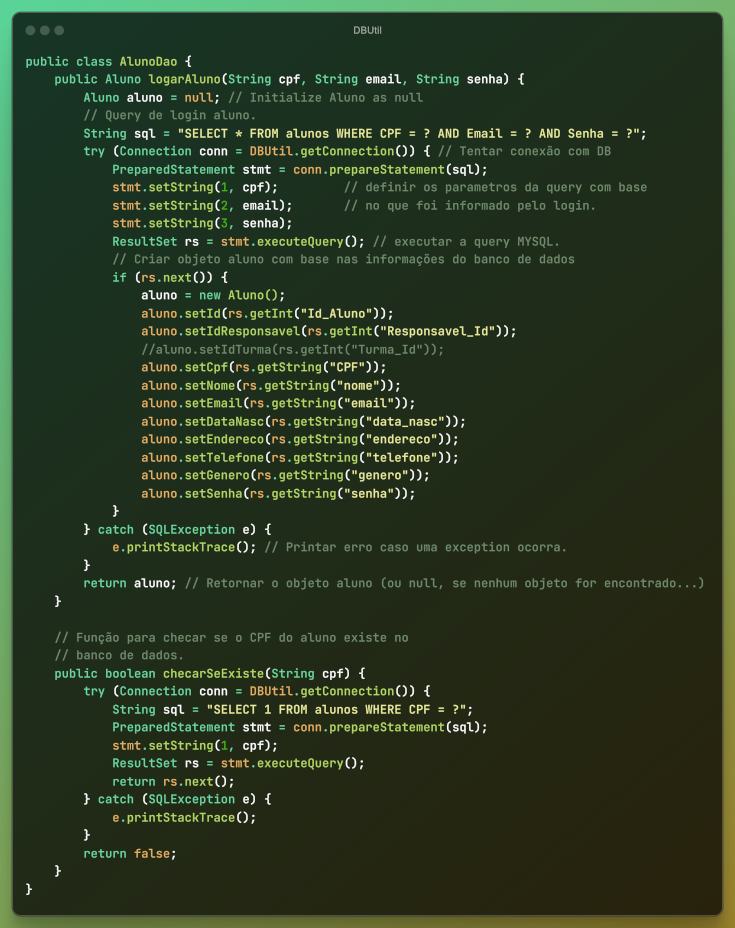
\includegraphics[scale=0.63]{imagens/code_scrs/3-loginaluno}
    \caption{DAO do Aluno}
\end{figure}

\begin{figure}[H]
    \centering
    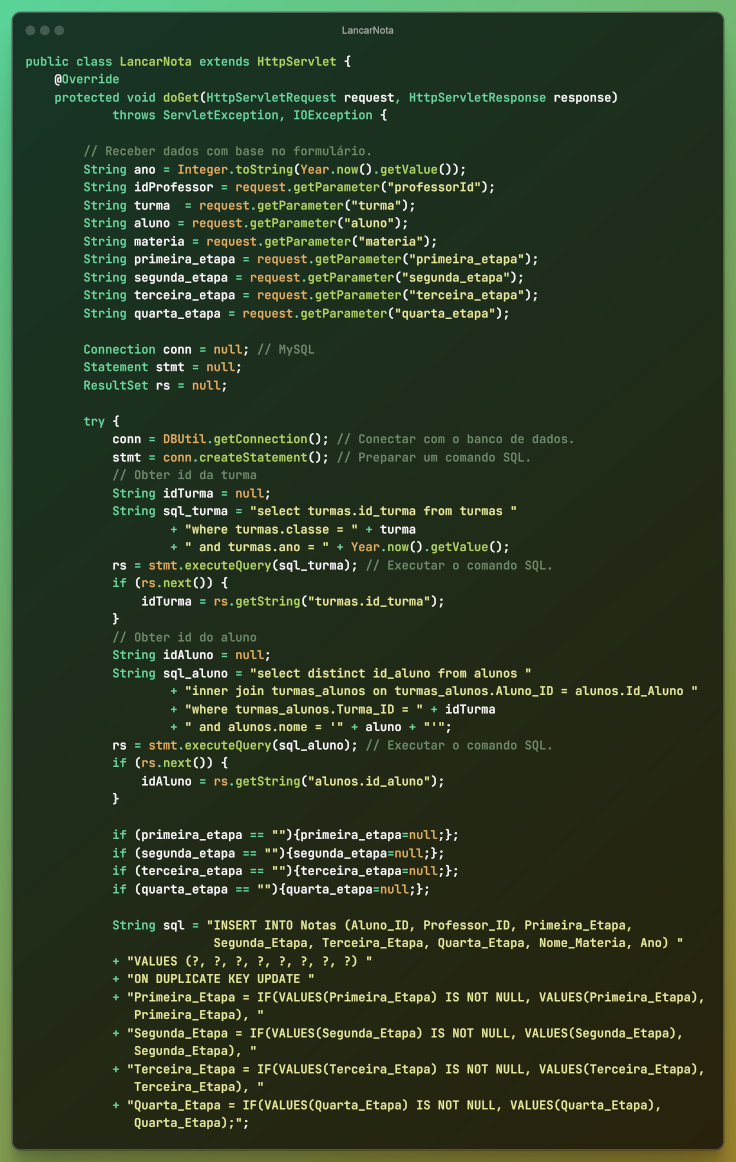
\includegraphics[scale=0.6]{imagens/code_scrs/4-lancarNota1.png}
    \caption{Lançamento de Nota pelos Professores (print n.1)}
\end{figure}

\begin{figure}[H]
    \centering
    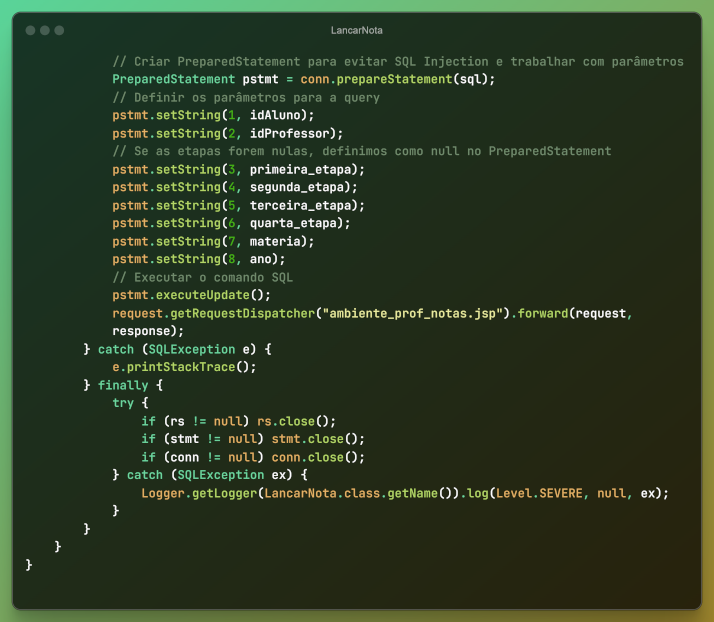
\includegraphics[scale=0.63]{imagens/code_scrs/5-lancarNota2.png}
    \caption{Lançamento de Nota pelos Professores (print n.2)}
\end{figure}

\begin{figure}[H]
    \centering
    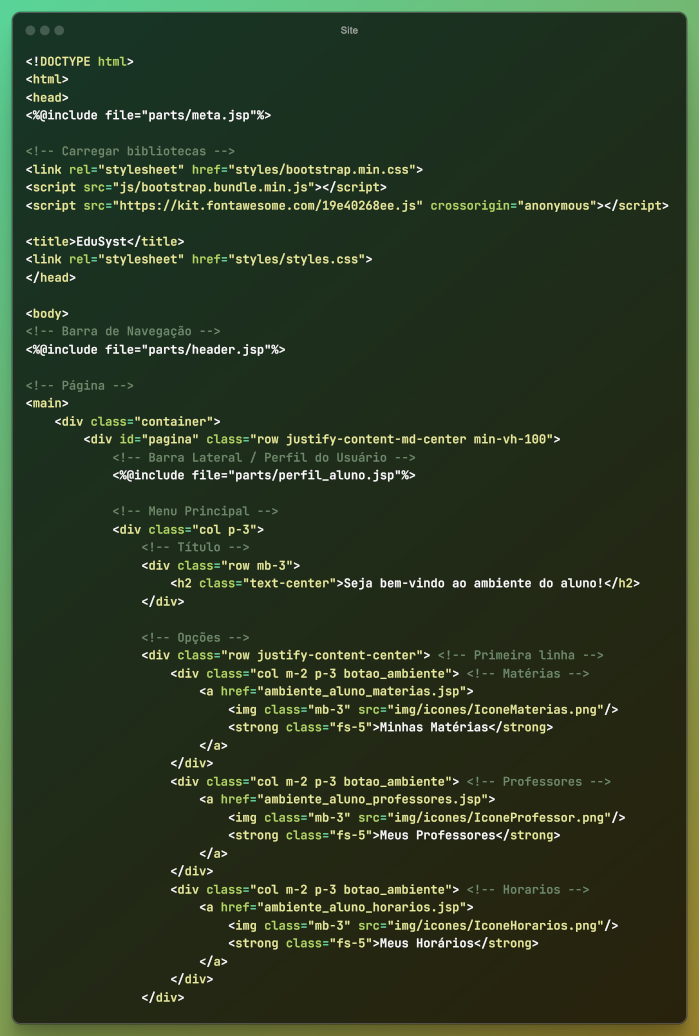
\includegraphics[scale=0.63]{imagens/code_scrs/6-ambienteSite}
    \caption{Ambiente do Usuário (print n.1)}
\end{figure}

\begin{figure}[H]
    \centering
    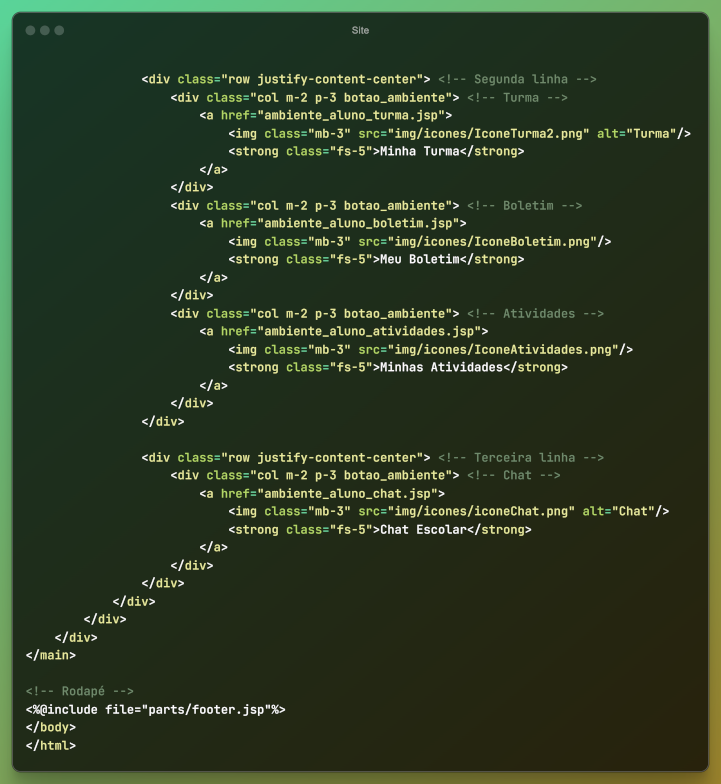
\includegraphics[scale=0.63]{imagens/code_scrs/7-ambienteSite2}
    \caption{Ambiente do Usuário (print n.2)}
\end{figure}

\subsection{Android Studio / Java / PHP}
\begin{figure}[H]
    \centering
    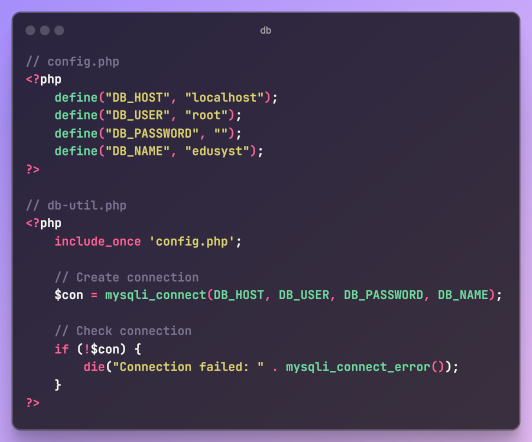
\includegraphics[scale=0.6]{imagens/code_scrs/8-andDb}
    \caption{Conexão com o Banco de Dados MySQL}
\end{figure}

\begin{figure}[H]
    \centering
    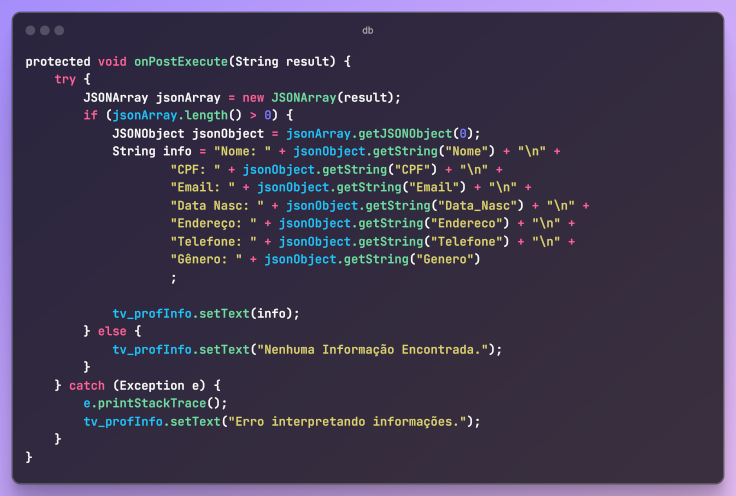
\includegraphics[scale=0.6]{imagens/code_scrs/11-obterProfInfo}
    \caption{Obter Informações de um Professor}
\end{figure}

\begin{figure}[H]
    \centering
    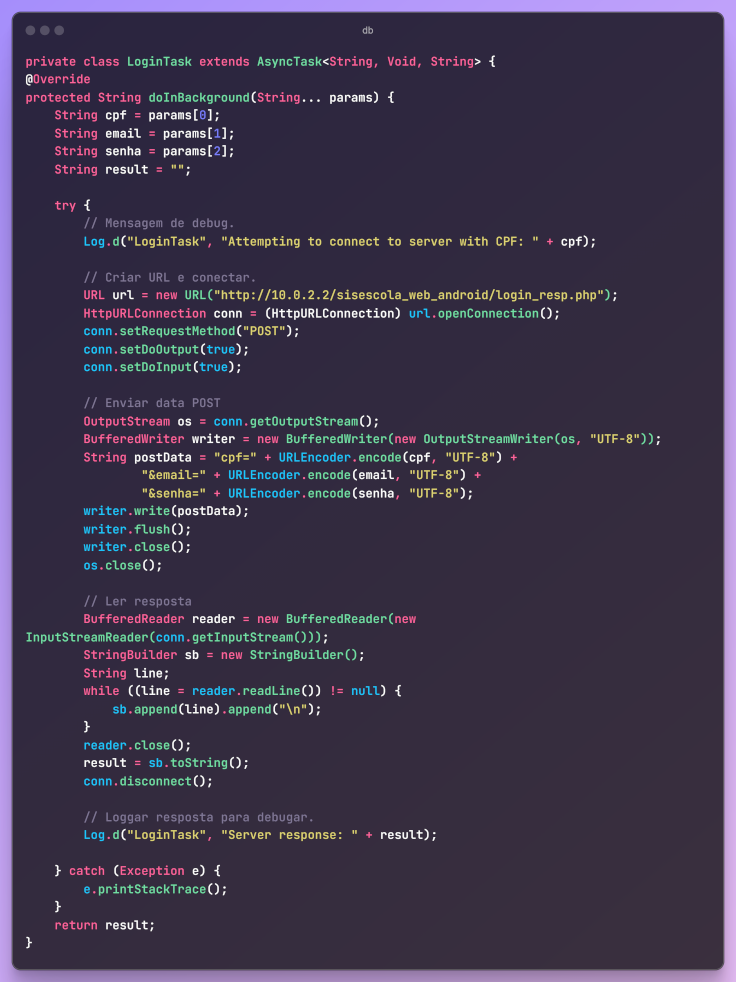
\includegraphics[scale=0.63]{imagens/code_scrs/9-loginResp}
    \caption{Login Responsável}
\end{figure}

\begin{figure}[H]
    \centering
    \includegraphics[scale=0.63]{imagens/code_scrs/10-Boletim}
    \caption{Geração do Boletim}
\end{figure}

\subsection{Java Desktop}
\begin{figure}[H]
    \centering
    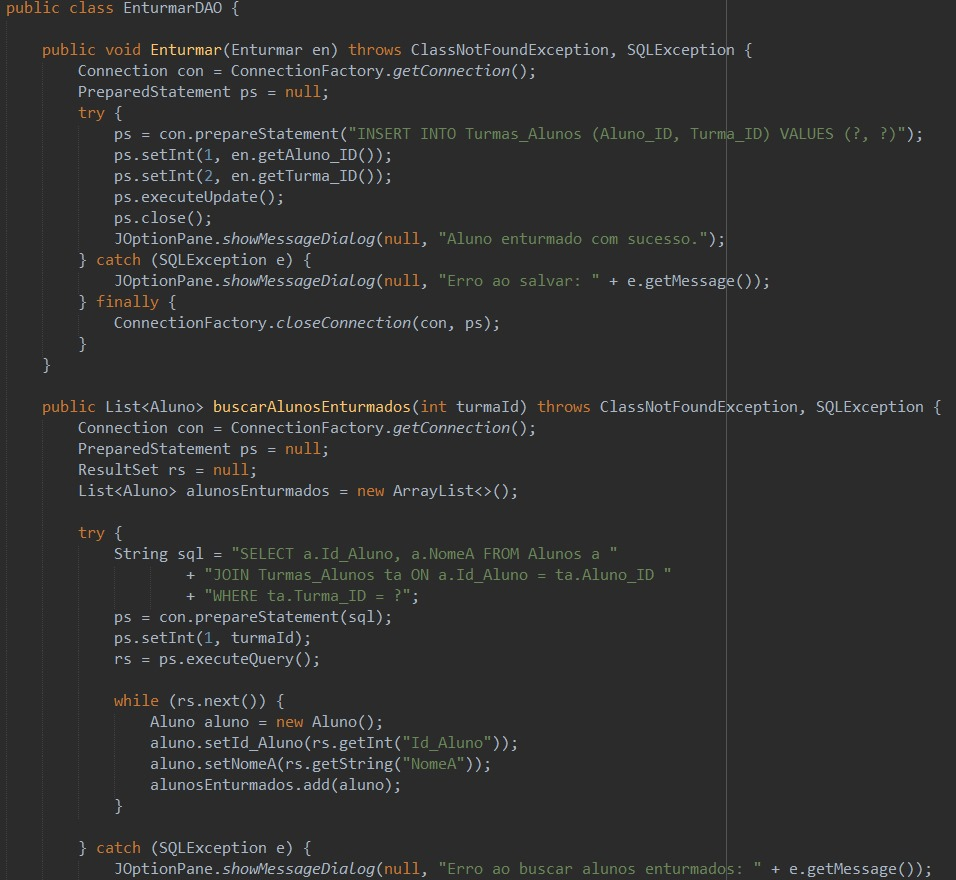
\includegraphics[scale=0.65]{imagens/code_scrs/12-enturmar}
    \caption{Enturmação}
\end{figure}

\begin{figure}[H]
    \centering
    \hspace*{-2.82cm} % Ajuste o valor para mover a imagem para a esquerda
    \centering
    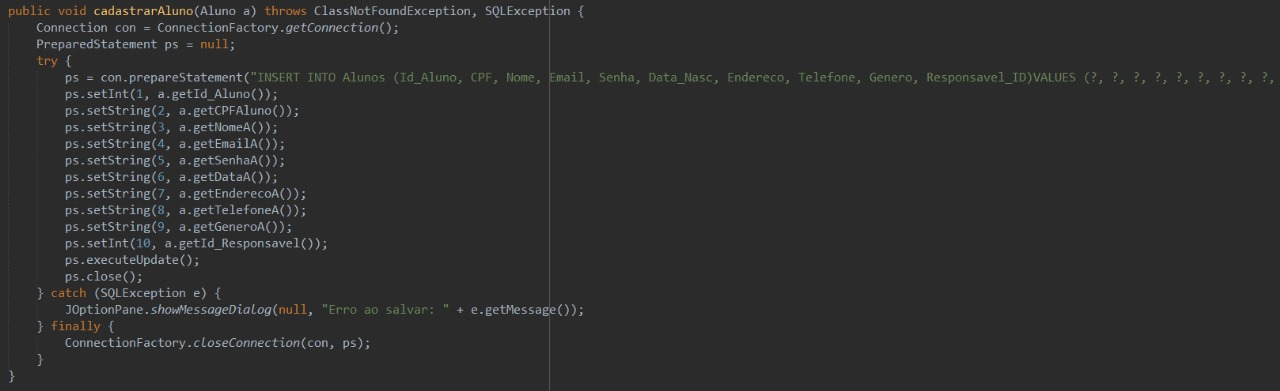
\includegraphics[scale=0.6]{imagens/code_scrs/13-cadastrarAluno}
    \caption{Cadastro de Alunos}
\end{figure}

\begin{figure}[H]
    \centering
    \hspace*{-2.82cm} % Ajuste o valor para mover a imagem para a esquerda
    \centering
    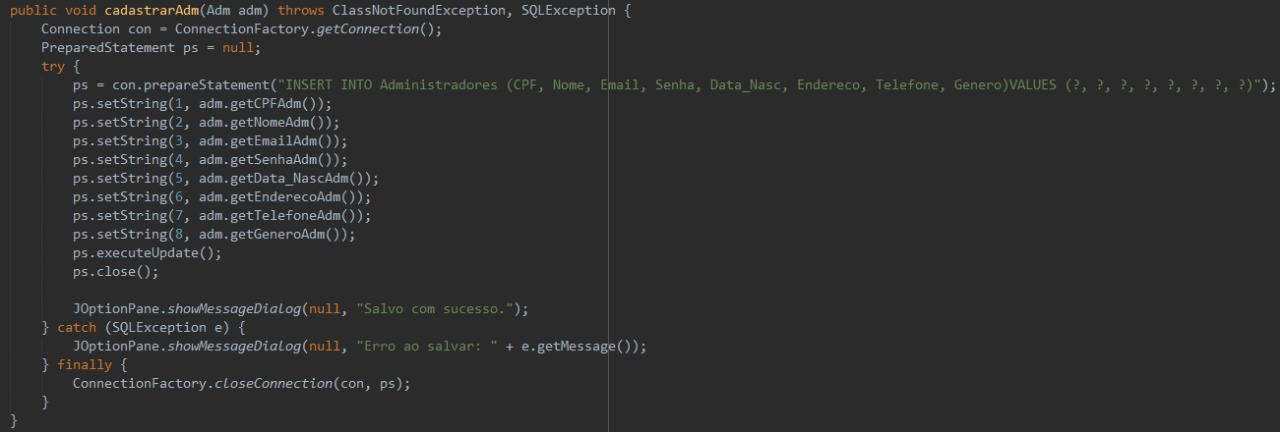
\includegraphics[scale=0.6]{imagens/code_scrs/15-cadastrarAdm}
    \caption{Cadastro de Turmas}
\end{figure}

\begin{figure}[H]
    \centering
    \hspace*{-2.82cm} % Ajuste o valor para mover a imagem para a esquerda
    \centering
    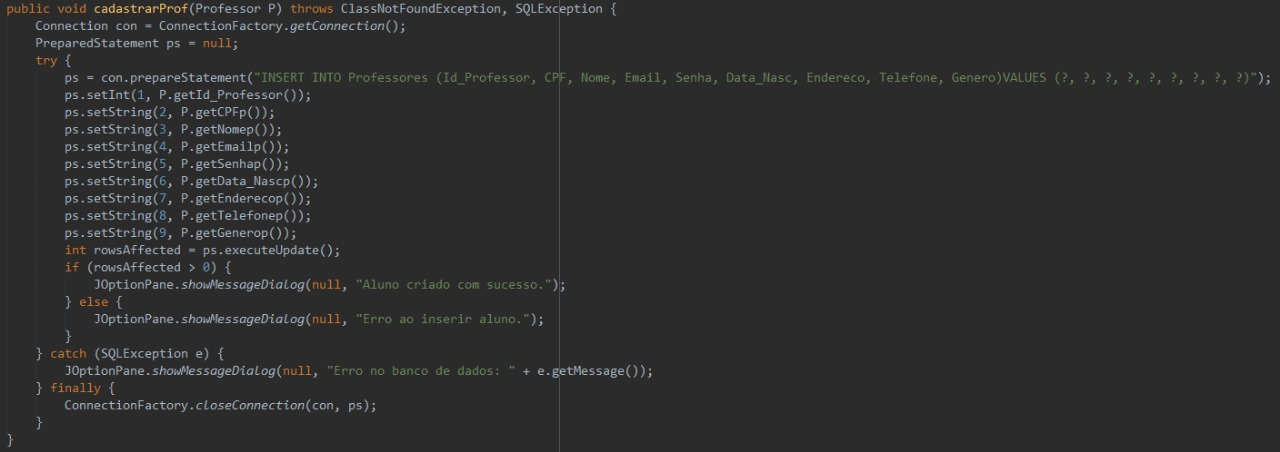
\includegraphics[scale=0.6]{imagens/code_scrs/17-cadastrarProf}
    \caption{Cadastro de Professores}
\end{figure}

\begin{figure}[H]
    \centering
    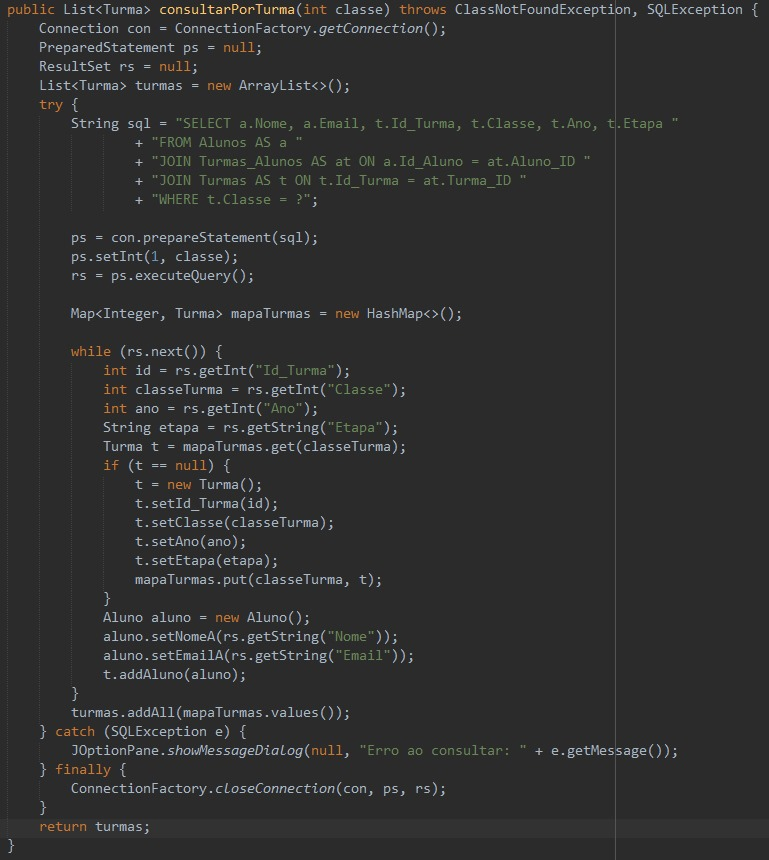
\includegraphics[scale=0.8]{imagens/code_scrs/14-listarTurma}
    \caption{Listagem de Turmas}
\end{figure}

\subsection{MySQL}
\begin{figure}[H]
    \centering
    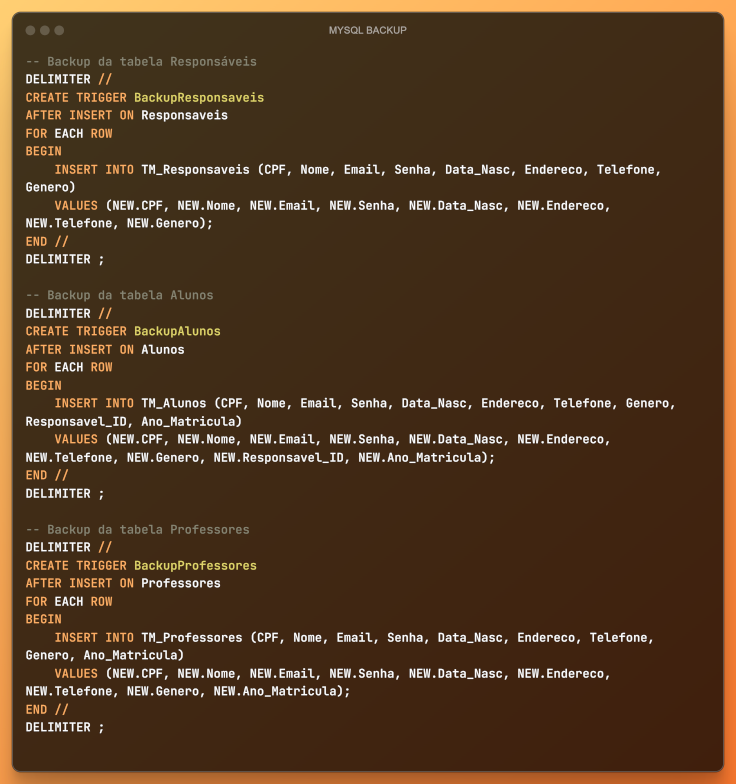
\includegraphics[scale=0.63]{imagens/code_scrs/1-mysql}
    \caption{Backup das Tabelas}
\end{figure}
% -------------------------------------------------------------------------------

% -------------------------------------------------------------------------------
\newpage
\section{Conclusão}
Ao final do desenvolvimento do EduSyst, foi possível consolidar um sistema funcional, voltado para apoiar a gestão escolar em escolas públicas, em especial as de ensino médio no estado do Rio de Janeiro. Nosso objetivo principal foi criar uma ferramenta que tornasse mais prática e organizada a comunicação e o acompanhamento de alunos, parentes e equipe escolar, e acreditamos ter dado um primeiro passo nesse sentido. Conscientes de que muitos aprimoramentos ainda são possíveis, principalmente no que diz respeito à segurança e à escalabilidade do sistema, concluímos esta etapa com a visão de que o EduSyst servirá como um alicerce, permitindo que melhorias futuras possam ser feitas e que mais escolas possam, aos poucos, se beneficiar de uma gestão digital mais estruturada e eficiente.

O desenvolvimento, embora desafiador, proporcionou um aprendizado intenso em programação, design de banco de dados e metodologias de desenvolvimento em equipe, consolidando um conhecimento essencial para a nossa formação. Este trabalho é um ponto de partida, e ficamos satisfeitos com o que conseguimos realizar até aqui. Esperamos que a plataforma contribua para o ambiente escolar e inspire outras iniciativas voltadas para a realidade das escolas públicas.
% -------------------------------------------------------------------------------

% -------------------------------------------------------------------------------
% \section{Scripts Sistema Desktop (Java SE)}
% \subsection{Scripts JAVA}

% \section{Scripts Sistema Web (Java EE)}
% \subsection{Scripts HTML}
%\subsection{Stylesheets CSS}
%\subsection{Scripts JSP}

%\section{Scripts Sistema Android (Android SDK)}
%\subsection{Scripts XML}
%\subsection{Scripts JAVA}
%\subsection{Scripts PHP}
% -------------------------------------------------------------------------------

\end{document}